\documentclass[letterpaper, 12pt]{article}


\usepackage{cmjStyle-pdftex} %use CMJ style
\usepackage{natbib} %natbib package, necessary for customized cmj BibTeX style
\bibpunct{(}{)}{;}{a}{}{,} %adapt style of references in text

% \doublespacing


\raggedright % use this to remove spacing and hyphenation oddities
%\setlength{\parindent}{0} % first para indent?
\setlength{\parskip}{2ex}
\parindent 24pt
\urlstyle{same} % make url tags have the same font
\setcounter{secnumdepth}{-1} % remove section numbering

\usepackage{ifpdf}

\DeclareGraphicsExtensions{.pdf,.png,.jpg}
\graphicspath{{../fig/}}


%% The package endfloat moves all floats (figures, tables...) to the end of the paper, as required for the final version of a CMJ paper.
%% Leave this package commented out for initial submission, but uncomment it for final version. 
% \usepackage{endfloat}

\usepackage{microtype}

%---Document----------
\begin{document}

{\cmjTitle 	Computation as material: (meta) live coding experiences}
\vspace*{24pt}

% (In the initial submission, omit all the following author information to ensure anonymity during peer review.)

%author - name
{\cmjAuthor Till Bovermann}
%author - address
\newline
\begin{cmjAuthorAddress}
	Media Lab Helsinki, Department of Media\\
	Aalto University\\
	H\"ameentie 135 c\\
	00560 Helsinki, Finland\\
	till.bovermann@aalto.fi
\end{cmjAuthorAddress}

\vspace*{24pt}
{\cmjAuthorPhone +358 (50) 5296398}
\vspace*{24pt}

%author - name
{\cmjAuthor Dave Griffiths}
%author - address
\newline
\begin{cmjAuthorAddress}
	FoAM\\
	Koolmijnenkaai 30-34\\
	1080 Brussels\\
	Belgium\\
	dave@fo.am
\end{cmjAuthorAddress}

\vspace*{24pt}
{\cmjAuthorPhone +32 2 5135928}
\vspace*{24pt}


% use of asterisk in section number to remove numbering
\section{Abstract}



\section{<<Start article>>}

% + how people imagine computation now (scary stuff) (Dave)

Computation is odd. 
In fact in many ways it's one of the strangest things that have been discovered, and 77 years on we continue to fail to fully grasp it's behaviour and so, struggle to keep unseen ramifications of our decisions under control. Faced with such a strange and yet essential beast the only sane strategy is to try and tame it. 
The field of software engineering is littered with concepts such as regression testing, type checking, white rooms, sandboxing, contracts, and encapsulation -- all attempts to cope with the fact that we can't really understand how a mundane machine of sufficient complexity will act when it is programmed by a human.

Livecoders look this beast straight in the eyes. 
When a livecoding performer takes to the stage and projects her screen, she invites us to join her in attempting to understand this intricate dance between human and machine. 

But livecoding is more than performance practice.
It is a broad field that can be viewed from many different angles.
From rehearsed public performances, reaching over collaborative improvisations and individual sound explorations, to it's utilisation as a method in science, it has been utilised in a manifold of applications.
All these derivations of the original theme share elements of live coding as they are featured in the toplap manifesto.
So livecoding is attempting to treat computation as a material on it's own terms, pick it up and feel what shapes it has.

Betablocker is an approach to livecoding which has brought to light many different strategies for presenting computation as a tangible material -- and it does this by making this process as much part of the performance as the code that describes it.
Built around this element is a variety of applications for testing, performing and scientific as well as artistic investigations.

Three levels: (a) technology, (b) unfolding as performance/research practice/method (conceptual and descriptive) and (c) aesthetic qualities.


This paper collects experiences, challenges and insights gathered by the two authors over the course of 3 years while investigating the combination of live coding techniques with virtual chips.

Soon after starting the project, it became evident that complex behaviour can emerge out of simple instructions and self-alteration of code.
Leading to a bunch of different insights

\subsection{disclaimers}
\label{sub:disclaimers}

The Betablocker computation does not make any distinction between a program (i.e., an instruction set) and data (i.e., data on which the program operates). 
The notions of code, data and program are therefore synonyms, however they represent semantical meaning rather than systematical/structural meaning.
Particular attention has to be given to the fact that, although a specific part of data stored on Betablocker's heap is meant to be a program, it is by definition possible that it is altered (e.g., by a separate process running independently on the same heap).

A state vector consisting of a heap, a stack and a program counter sufficiently represents the state of a Betablocker engine.

\parskip 18pt

\section{BetaBlocker core technology} 
\label{sec:betablocker_core}

% describing the theoretical background and implementation (switch statement etc.)

The Betablocker core is a simple multithreaded virtual machine following the \emph{von Neumann architecture} design pattern where there is no separation between code and data.
It's uncrashable, so every possible program will run, although it will halt in infinite loops. 
It has 23 instructions whose width is either 8 or 16bit for those that take operands. The heap is constrained to 256 bytes of memory, while each thread has 8 bytes of stack. 


BetaBlocker has the following structure:(a) a heap of 256 8bit values, (b) an instruction table, (c) a process consisting of (ca) a program counter, pointing to an address in the heap, and (cb) a stack of eight 8bit values.

\subsection{Heap} 
\label{sub:heap}
This is the place where the program and its data are located. In line to the von Neumann architecture, it is possible (and intended) to alter the program while it is running, i.e. interpreting it as data rather than an instruction set. The actual representation of a heap is an array of 256 8bit values. Each value can be interpreted either as an instruction, an address, or an actual number.


\subsection{Thread} 
\label{sub:thread}
A thread is something that executes code stored on the heap. It has a current position (the instruction it is currently evaluating), a stack (some sort of storage, see below), and a timer, determining when it will move its program counter to the heap's next address.

\subsection{Stack} 
\label{sub:stack}
A stack serves as a temporary storage for a thread. It can be accessed only from top by either (a) pop an item from the stack, (b) return the topmost item without removing it, and (c) push a value to the stack.


\subsection{Instruction set} 
\label{sub:instructions}

% TODO: IMHO, we should differenciate between a core instruction set (without e.g. NOTE and VOX) and various add-ons (NOTE, VOX, OUT).

These are the implemented instructions:

\begin{description}
\item[\texttt{NOP}] do nothing
\item[\texttt{ORG}] define relative origin address for this thread
\item[\texttt{EQU}] compare first two elements on the stack, pop them off the stack, and push the result
\item[\texttt{JMP}] jump to the address specified right after this instruction
\item[\texttt{JMPZ}] jump only if stack returns 0
\item[\texttt{PSHL}] push value on address specified right after this instruction to the stack
\item[\texttt{PSH}] push value on address specified by the value on the address specified right after this instruction to the stack
\item[\texttt{PSHI}] like push but one more encapsulation
\item[\texttt{POP}] pop item from stack to the point in the heap following this instruction
\item[\texttt{POPI}] pop item from stack and write the value at that address in the heap to the address following this instruction
\item[\texttt{ADD}] perform an addition on the first two elements on the stack, pop them off the stack, and push the result
\item[\texttt{SUB}] perform a subtraction on the first two elements on the stack, pop them off the stack, and push the result
\item[\texttt{INC}] increment value on stack
\item[\texttt{DEC}] decrement value on stack
\item[\texttt{AND}] perform a bit-wise "and" on the first two elements on the stack, pop them off the stack, and push the result
\item[\texttt{OR}] perform a bit-wise "or"" on the first two elements on the stack, pop them off the stack, and push the result
\item[\texttt{XOR}] perform a bit-wise "xor" on the first two elements on the stack, pop them off the stack, and push the result
\item[\texttt{NOT}] perform a bit-wise "not" on the first element on the stack, pop it off the stack, and push the result
\item[\texttt{ROR}] perform a right shift operation on the first two elements on the stack, pop them off the stack, and push the result
\item[\texttt{ROL}] perform a left shift operation on the first two elements on the stack, pop them off the stack, and push the result
\item[\texttt{PIP}] increments value specified by the next value on the heap
\item[\texttt{PDP}] decrements value specified by the next value on the heap
\item[\texttt{DUP}] push a duplicate of the topmost value of the stack to the stack
\item[\texttt{NOTE}] (DS extension) play a note
\item[\texttt{VOX}] (DS extension) play a vox
\item[\texttt{OUT}] (spork factory extension) pops the top of the stack and writes it to the pins on % \item[\texttt{STOP}] stop program (here: like NOP)
an ATtiny
\end{description}
This is their actual implementation:

\begin{Verbatim}[fontfamily=courier, xleftmargin=\parindent]
switch(instr)
{
case  NOP: break;
case  ORG: m_start=m_start+m_pc-1; m_pc=1; break;
case  EQU: push(pop()==pop()); break;
case  JMP: m_pc=peek(m,m_pc++); break;
case JMPZ: m_pc++; if (pop()==0) m_pc=peek(m,m_pc); break;
case PSHL: push(peek(m,m_pc++)); break;
case  PSH: push(peek(m,peek(m,m_pc++))); break;
case PSHI: push(peek(m,peek(m,peek(m,m_pc++)))); break;
case  POP: poke(m,peek(m,m_pc++),pop()); break;
case POPI: poke(m,peek(m,peek(m,m_pc++)),pop()); break;
case  ADD: push(pop()+pop()); break;
case  SUB: push(pop()-pop()); break;
case  INC: push(pop()+1); break;
case  DEC: push(pop()-1); break;
case  AND: push(pop()&pop()); break;
case   OR: push(pop()|pop()); break;
case  XOR: push(pop()^pop()); break;
case  NOT: push(~pop()); break;
case  ROR: push(pop()>>peek(m,m_pc++)); break;
case  ROL: push(pop()<<peek(m,m_pc++)); break;
case  PIP: 
{ u8 d=peek(m,m_pc++);
  poke(m,d,peek(m,d)+1);
} break;
case  PDP:
{ u8 d=peek(m,m_pc++);
  poke(m,d,peek(m,d)-1);
} break;
case  DUP: push(top()); break;
default : break;
};
\end{Verbatim}


\section{Background and historical context} 
\label{sec:background}

% musical and computational

Betablocker was the first attempt at a game pad programmable live coding system in fluxus. 
It was inspired by a discussion on the TOPLAP mailing list about virtual machines, and also visually by games such as "Mr Driller," in terms of colourful blocks interacting with each other and setting up chain reactions as a game mechanic.

The program is a virtual machine running inside fluxus. 
It visualises the simulation of a fictional CPU with 256 bytes of memory, and allows multiple threads of execution to be run sharing the same address space. 
The Betablocker language is very much based on the ideas in Core Wars,

From a musical point of view, Betablocker can be viewed as a tool for algorithmic composition (\cite{maurer1999-a-b}).

Betablocker/Audio: Formalized Music: mathematical/stochastic sound synthesis, Gendy (\cite{Xenakis:1971}, \cite{luque2009-the}).



\section{Distinct character of Betablocker and its influence on sound and performance practice} 
\label{sec:distinct_character}


% \subsection{Computational features} 
% \label{sub:computational_features}

BetaBlocker is distinct to other approaches of computational machines in several aspects:
In the design of Betablocker, the ability to observe computational behaviour was an essential goal, whereas the result of the computation (and therefore process optimisation) played a minor role.  
Furthermore, Betablocker is implemented as a software emulation and can be modified easily.
This allows for its alteration regarding introspection (by adding probes) and customisation (by altering the instruction set).
Last not least, compared to common microprocessor architectures such as the x86\footnote{\url{http://en.wikipedia.org/wiki/X86}}, AVR\footnote{\url{http://en.wikipedia.org/wiki/Atmel_AVR}} or RISC\footnote{\url{http://en.wikipedia.org/wiki/Reduced_instruction_set_computing}}, Betablocker's architecture is simplistic.
Operational complexity arises from the induced data and its processing rather than from the system's architectural features.

The character of Betablocker influences not only the sonic results of a livecoding session but also its overall structuring.
Due to its potential process complexity, it is e.g. possible to start with a blank page\footnote{As proposed in the TOPLAP Manifesto draft published at \url{http://toplap.org/wiki/ManifestoDraft}.}
and add a fairly complicated pattern as the next step.

We describe our findings and explorations with regard to Betablocker in the next paragraphs and give insights on how its behaviour influenced our livecoding sessions.
As we used Betablocker mainly in two perceptional contrasting settings, rhythmic and sonic, we differentiate in the following between Betablocker/Slow and Betablocker/Audio.


% rythmical patterns vs. audiosynthesis
\subsubsection{Slow computing -- Betablocker/Slow}
\label{sub:slow_computing}
%  describing the nintendoDS part of the implementation
It began as a highly graphical fluxus based livecoding environment to be performed with the use of a gamepad (debuted at Piksel Festival 200something) and later moved on to the Gameboy DS in order to make use of it's particular graphics processing, sound chip and stylus input method -- while the small screen on the device is projected by the use of a webcam.

% TODO: more detail, also technical level... graphical interface, why you chose the grid gui etc.

Betablocker/Slow (the Fluxus/DS version) makes computation tangible by slowing down processes by many orders of magnitude compared to typical scenarios. 
The smallest musical loop in Betablocker/Slow is 3 instructions long -- push a value onto the stack (\texttt{PSH, 123}), play it as a note (\texttt{NOTE}), jump back to start (\texttt{JMP 0}). 
In order to play this at 120 BPM it will need to run at 6 cycles per second, the machine I am typing on peaks at $2.8*10^9$ cycles per second, which is 466 million times faster than Betablocker/Slow. This makes computation audible as techno music, and simultaneously visible as the thread's positions are displayed on the livecoding interface synced with the audio along with the entire heap's memory contents - forming a complete state vector of the processor.

Performing with Betablocker/Slow consists of starting with empty memory and manually writing programs that modify themselves and each other.
Eventually the quantity of self replicating fork bombs, sequencers interpreting memory as percussion synth triggers and programs busily reversing the contents of memory reaches a level where the performer is confronted with a Turing soup which is happily writing it's own code. 
At this point the decision is whether to collaborate or compete.
Collaboration involves looking for interesting bits of code that emerge and manually modifying them, while the best strategy for competing is attempting to find a space to write a program that gradually clears memory so you can start again. 
In most successful performances both choices are made over the course of the concert.



Some useful Betablocker DS code patterns as used in common live coding situations.
Firstly, when carrying out a sound check before a live performance it's important to keep some kinds of sound engineers happy generating as many different sounds as you can so they can fiddle around with stuff - of course remember to turn everything up to 8 when asked to make the loudest sound you can in order to leave some overhead to blow the PA.
This is a betablocker program which will play all the sounds in a sound bank at all frequencies. Add more concurrent threads to make it more interesting. Values interpreted as pointers are visualised as arrows:


\begin{figure}
	\centering
		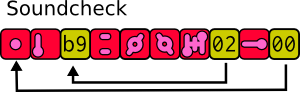
\includegraphics[width=13cm]{bbds-sndchk1}
	\caption{Sound check}
	\label{fig:fig_bbds-sndchk1}
\end{figure}

In betablocker the beat is always locked to the instruction cycle rate, so fast changing sounds are a matter of optimisation. One of the most common ways around this (and a good way to start things off in a gig) is to use one fast loop program for playing sounds while another slower program modifies the first by overwriting bits of it. 

\begin{figure}
	\centering
		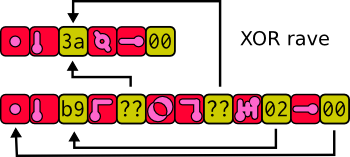
\includegraphics[width=13cm]{bbds-xorrave}
	\caption{XOR rave}
	\label{fig:fig_bbds-xorrave}
\end{figure}

Following on from the last installment of Betablocker DS coding patterns, this time looking at some very short programs that are nicely controllable by the livecoder - including some actual audio examples here (embedding seems broken on archive.org).
Both these example programs are 16 bytes long, and require 3 concurrent threads to be running over different parts of the program. Each thread has a simple purpose, the first loads a byte and plays it as a sound repeatedly, the second one increments the byte that the first is playing, and the third periodically resets the byte to a constant value.
 
\begin{figure}
	\centering
	% TODO: caption
		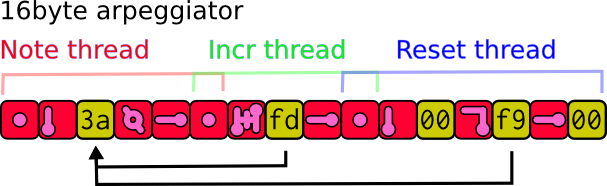
\includegraphics[width=13cm]{bbds-arp}
	\caption{XOR rave}
	\label{fig:fig_bbds-arp}
\end{figure}

The first example simply plays the byte as a note - resulting in an arpeggiator style sound. After writing the code, the performer can change the speed of each of the three threads to get quite a bit of variety. For example, the slower the resetting thread runs, the longer the pattern will be before it repeats.

\begin{figure}
	\centering
		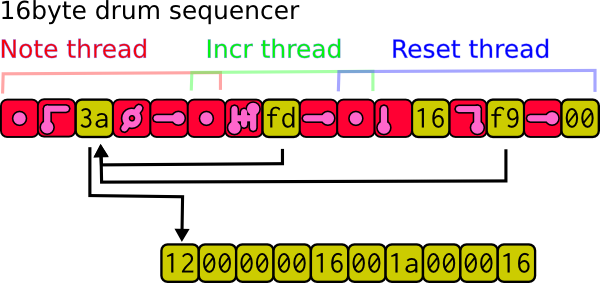
\includegraphics[width=13cm]{bbds-seq}
	\caption{XOR rave}
	\label{fig:fig_bbds-seq}
\end{figure}

The second example is very similar, but is slightly modified to play a sequence of different sounds rather than notes, to become a drum sequencer. The second instruction is also changed from a "push literal" to a "push contents of address" which results in the program playing a part of memory as a sequence. We can control the start address location with the reset byte, write directly to this part of memory, and fiddle with the other thread's speed to get even more complexity.



\subsubsection{Sound computing -- Betablocker/Audio} 
\label{sub:sound_computing}
%   + SuperCollider (Till)

Betablocker/Audio utilises the Betablocker engine to render sound directly by running it in the range of audio rate.
In the first attempt (the SuperCollider UGen implementation), process monitoring was a desired feature. 
We therefore added probes to specific parts of the engine.
As shown below, signal variety is therefore limited and influenced by its computation.

In a second attempt, Spork Factory, an additionally introduced instruction (\texttt{OUT}) writes out the topmost value on the stack.
In difference to the probing approach, this feature decouples sound output from computation, however requires faster execution rates to produce the same output.\footnote{Each instruction \texttt{I} that changes the stack has to be replaced by \texttt{[I, DUP, OUT]}}
In the next paragraphs, we will describe the implementation and implications of the first attempt.

We implemented Betablocker/Audio in SuperCollider for easy access not only in livecoding settings.\footnote{Available as open source code at \url{https://github.com/supercollider/sc3-plugins}.}
To facilitate typical usage, we decided to provide two different interfaces, a demand-rate UGen (\texttt{DetaBlockerBuf}) exposing the topmost value of the stack by means of SuperCollider's demand chain implementation and a multi-out version (\texttt{BBlockerBuf}) that exposes the position of the program counter as well as all 8 elements of the stack.
A basic example for their usage is given in the following listings.\footnote{It is assumed that the heap to be operated on is pre-loaded into a Buffer object.}
By adding the LeakDC operator to the stack values, possible DC offsets are prevented to affect the speaker system.

\begin{Verbatim}[fontfamily=courier, xleftmargin=\parindent]
x = { // BBlockerBuf example
	var signal = Demand.ar(
	  Impulse.ar('bbRate'.kr(22100)), 
	  'reset'.tr(0),
	  DetaBlockerBuf('heapBuf'.kr(0))
	);
	LeakDC.ar(signal);
}.play;
\end{Verbatim}

\begin{Verbatim}[fontfamily=courier, xleftmargin=\parindent]
x = { // BBlockerBuf example
	var pC, stack;
	#pC ... stack = BBlockerBuf.ar('bbRate'.kr(22100), 
		'heapBuf'.kr(0), 'startpoint'.kr(0));
	stack = LeakDC.ar(stack);
	 // use information on program counter to place sound output
	Splay.ar(stack, spread: 0.1, center: pC);
}.play;
\end{Verbatim}


\subsection{Sonic features} 
\label{sub:sonic_features}

% synthesis/human creation

\subsubsection{Noise aesthetics -- on texture and rhythm} 
\label{sub:noise_aesthetics}

% playing random instruction sequences vs. "conscious" programming
Although the system is deterministic, i.e., its outcome can be calculated supposed its state is known.
Due to it's complexity a valid and, as it turned out, fruitful approach is to work with randomness and empirical observations rather than with analytical approaches.

% analysis/findings
Random programs settle into a local stability. there is less high frequencies in the output signal. 
Sonic variation in random synthesis depends on time: 
first 1000 computation steps could be seen as transiental, whereas a longterm adaption takes place as sound settles over the course of several minutes to be less sharp/rough.

\subsubsection{Manually programming sonic structures}
\label{sub:manual_programming_sonic_structures}

When dealing with a computational system on a low level, the understanding of it's inner works is crucial.
With the given instructionset of Betablocker/Audio, we hand-crafted algorithms to produce specific waveforms as good as possible.
The simplest set is a sawtooth which can be implemented with the heap \texttt{[ORG, INC, JMP, 1]}.
An impulse at nearly Nyquist frequency can be rendered with the program \texttt{[ORG, NOT, JMP, 1]}, whereas a pulsewave with adjustable pulsewidth can be programmed with \texttt{[ORG, NOP, ... , NOT, JMP, 1]}.
More complex structures are a combination of a sawtooth and an impulse generator with adjustable slope of the sawtooth: \texttt{[ORG, PSHL, 6, ADD, JMP, 1, <slope>]}. Note that position 6 will never be reached by the program counter and therefore serves as a safe "data storage" for the slope value.
An overview of the rendered signals can be found in Figure~\ref{fig:fig_waveforms_POPdestroy-random}.

% POP destroy ( leak = false leak = true )
\texttt{[6, 7, 6, 245, ORG, NOP, NOP, NOP, NOP, PSHL, -6, PSHL, -2, POP, JMP, 1]}
If the remaining part of the heap is initialised with random values, a random number is pushed onto the stack.
% TODO: explain behavior...

\begin{figure}
	\centering
		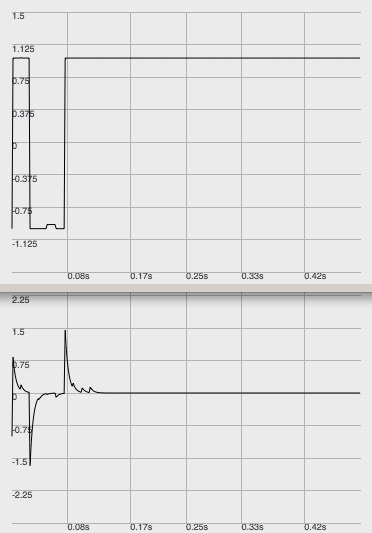
\includegraphics[width=5cm]{wv-POPdestroy-noRandom}
		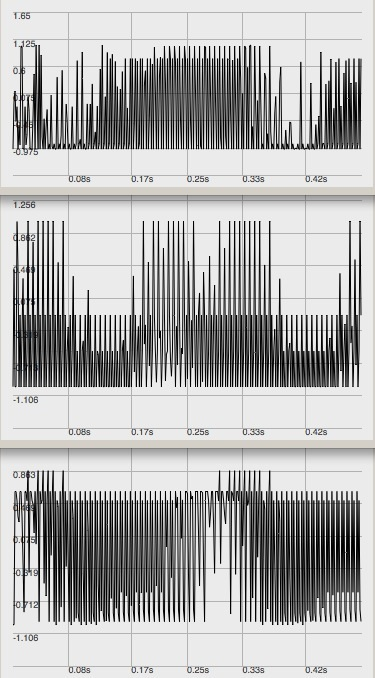
\includegraphics[width=5cm]{wv-POPdestroy-random}
		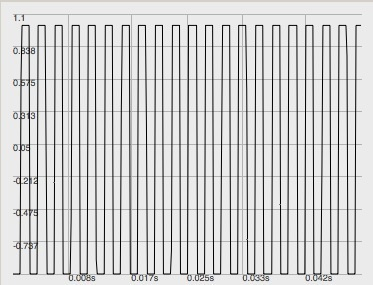
\includegraphics[width=5cm]{wv-impulse}
		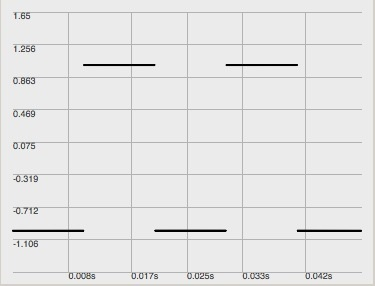
\includegraphics[width=5cm]{wv-pulse202}
		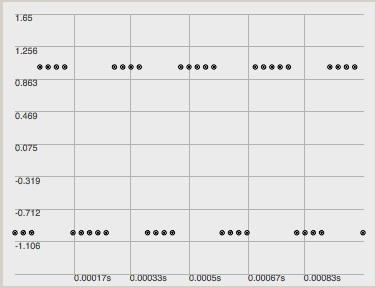
\includegraphics[width=5cm]{wv-pulse22}
		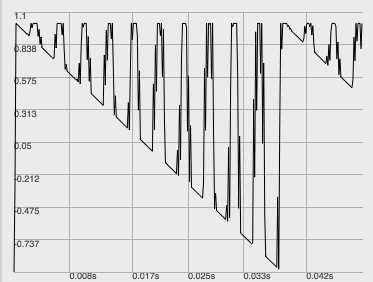
\includegraphics[width=5cm]{wv-sawImpulse}
		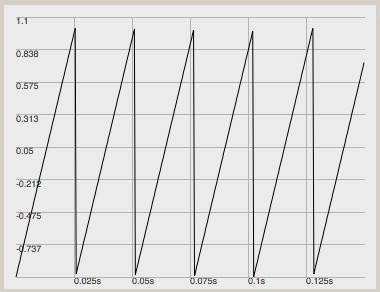
\includegraphics[width=5cm]{wv-sawtooth}
	\caption{All the waveforms generated manually}
	\label{fig:fig_waveforms_POPdestroy-random}
\end{figure}


%   + limitations and sonic characteristics of betablocker assembler programs
% TODO: find appropriate link to upper part
Findings: The shape of the waveform is limited due to the way the sound signal is derived from the Betablocker engine, namely probing the items on one of its functional parts, the stack. 
However, this limitation is inherent to the structure of the system itself.





\subsubsection{Classic synthesis techniques adapted to Betablocker} % (fold)
\label{sub:classic_synthesis_techniques_adapted_to_betablocker}

The Betablocker/Audio implementation allows for alteration of calculation rate. 
This opens the possibility to add dynamics not only in amplitude but also in pitch by FM/AM-like synth designs.
The following listings show examples on additive synthesis, frequency modulation and amplitude modulation of several Betablocker/Audio engines.
Implementation is done in SuperCollider.

% \begin{figure}
% 	\centering
% 		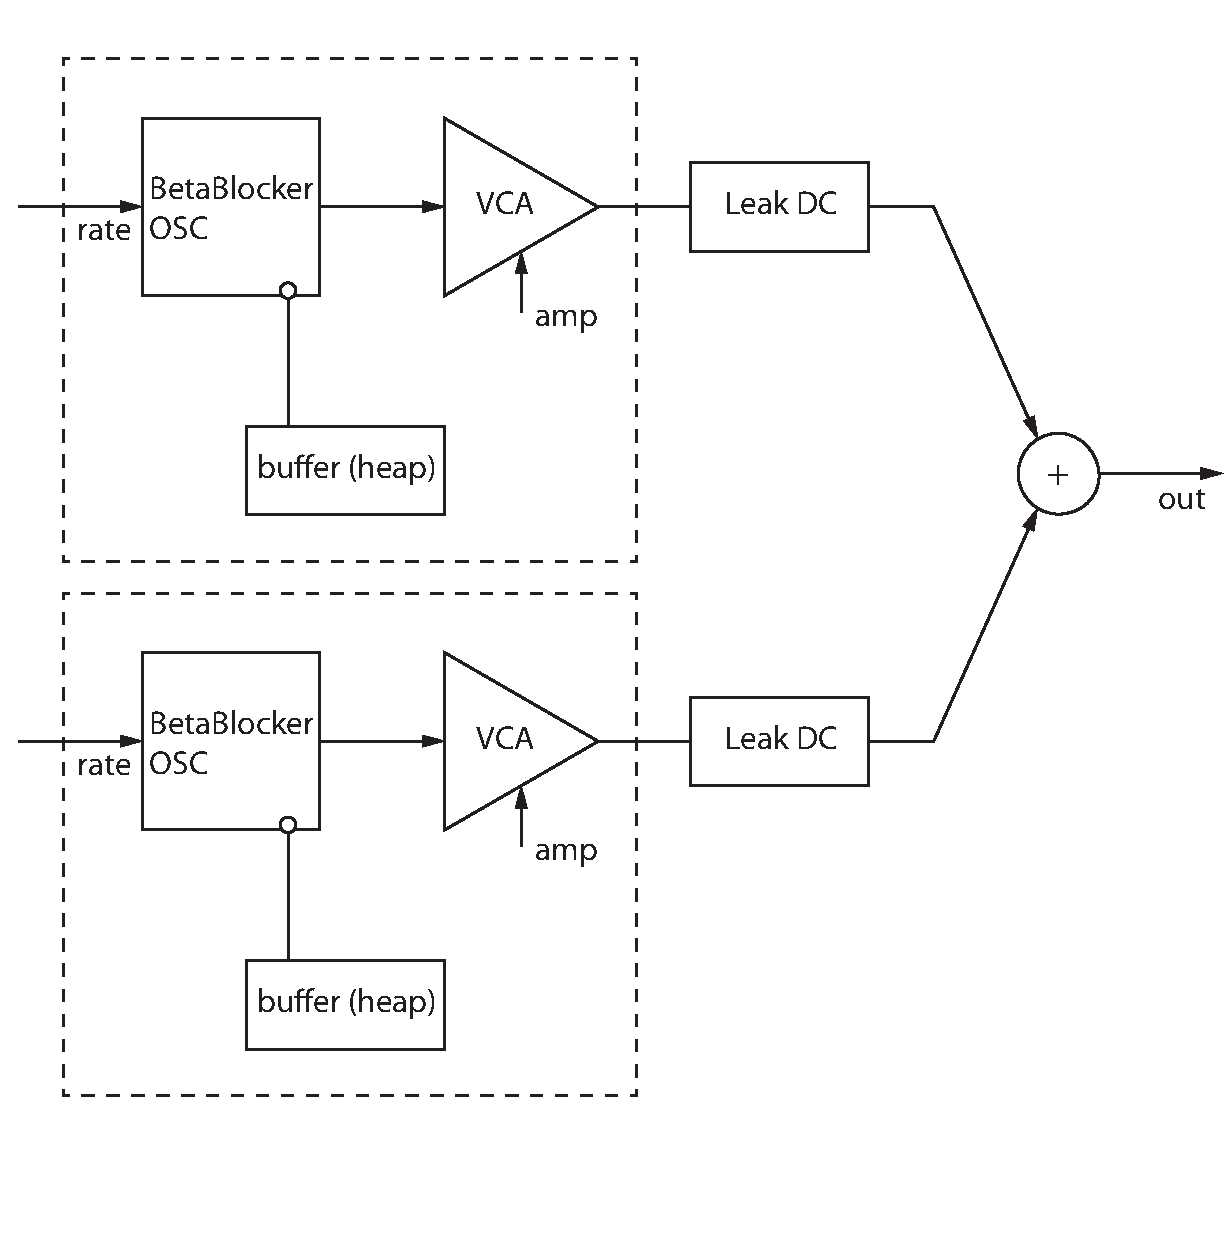
\includegraphics[height=3in]{Additive-Betablocker}
% 	\caption{Additive synthesis.}
% 	\label{fig:fig_Additive-Betablocker}
% \end{figure}
% \begin{figure}
% 	\centering
% 		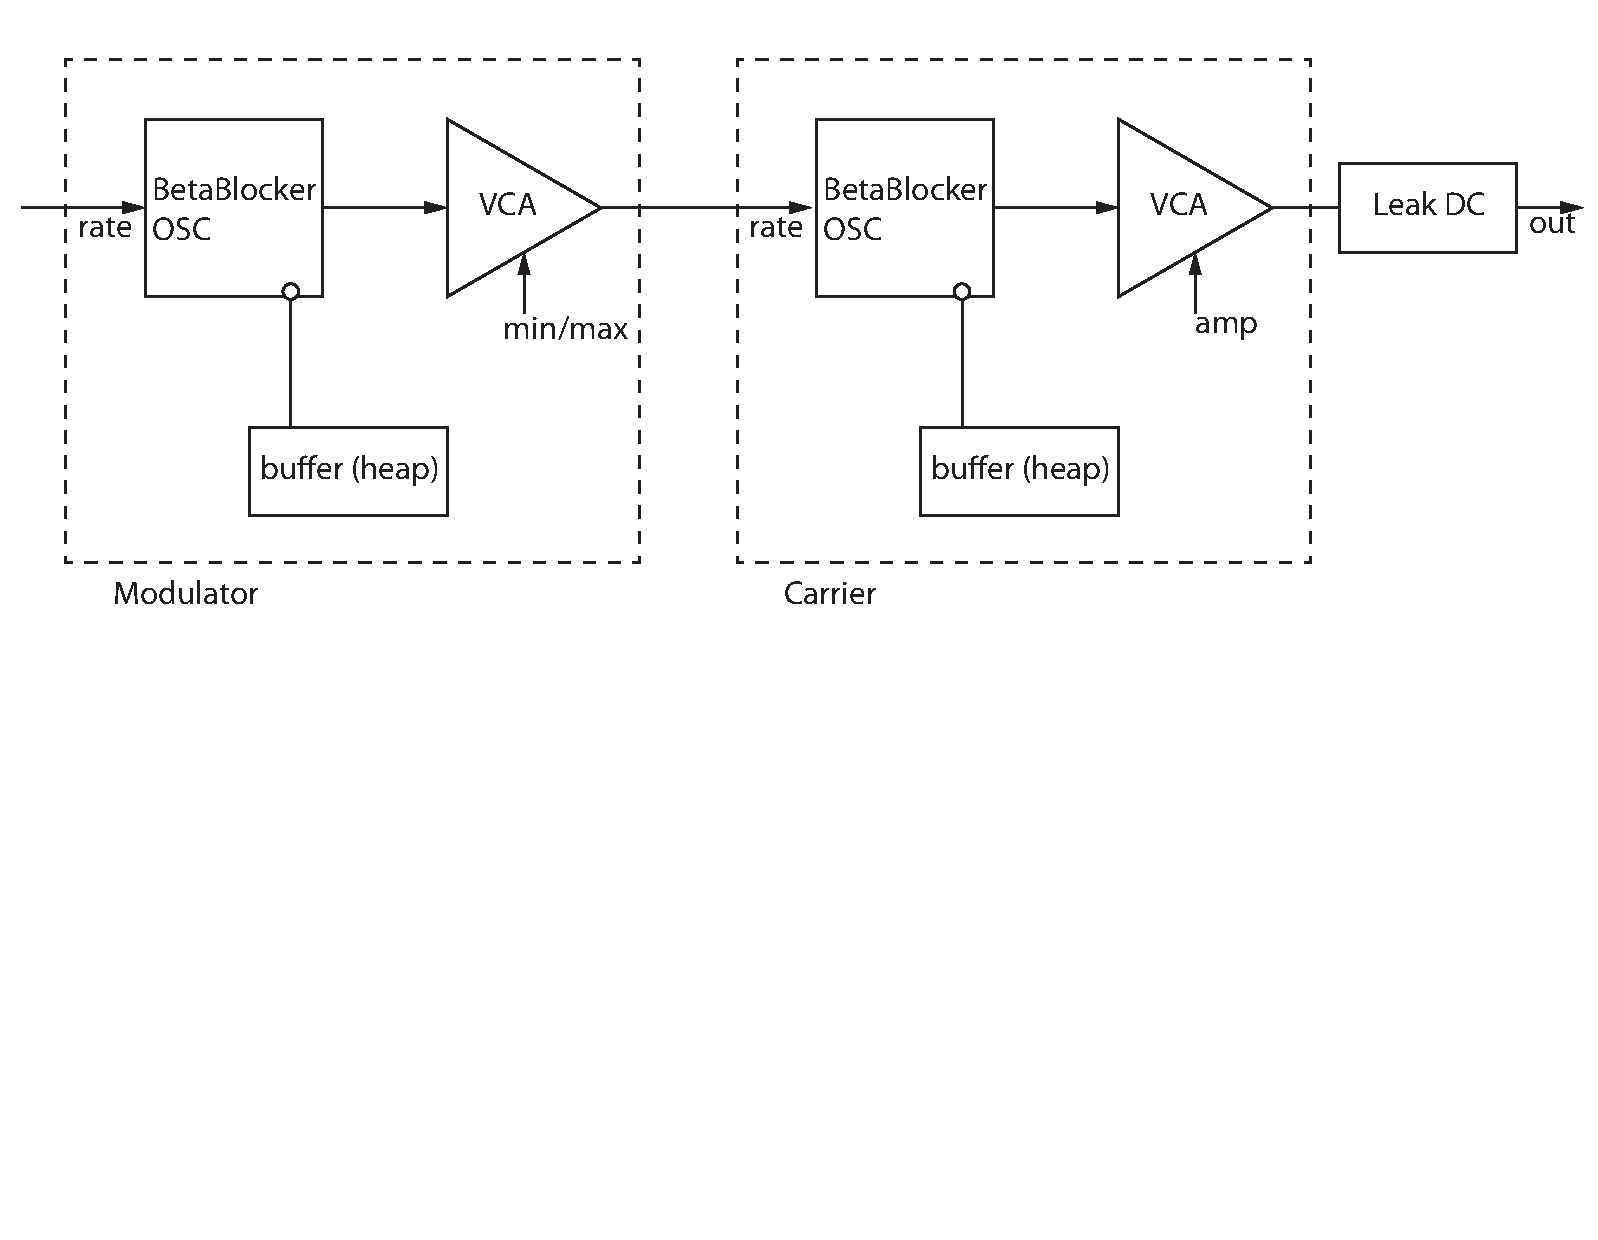
\includegraphics[height=3in]{FM-Betablocker}
% 	\caption{Frequency modulation synthesis.}
% 	\label{fig:fig_FM-Betablocker}
% \end{figure}
% \begin{figure}
% 	\centering
% 		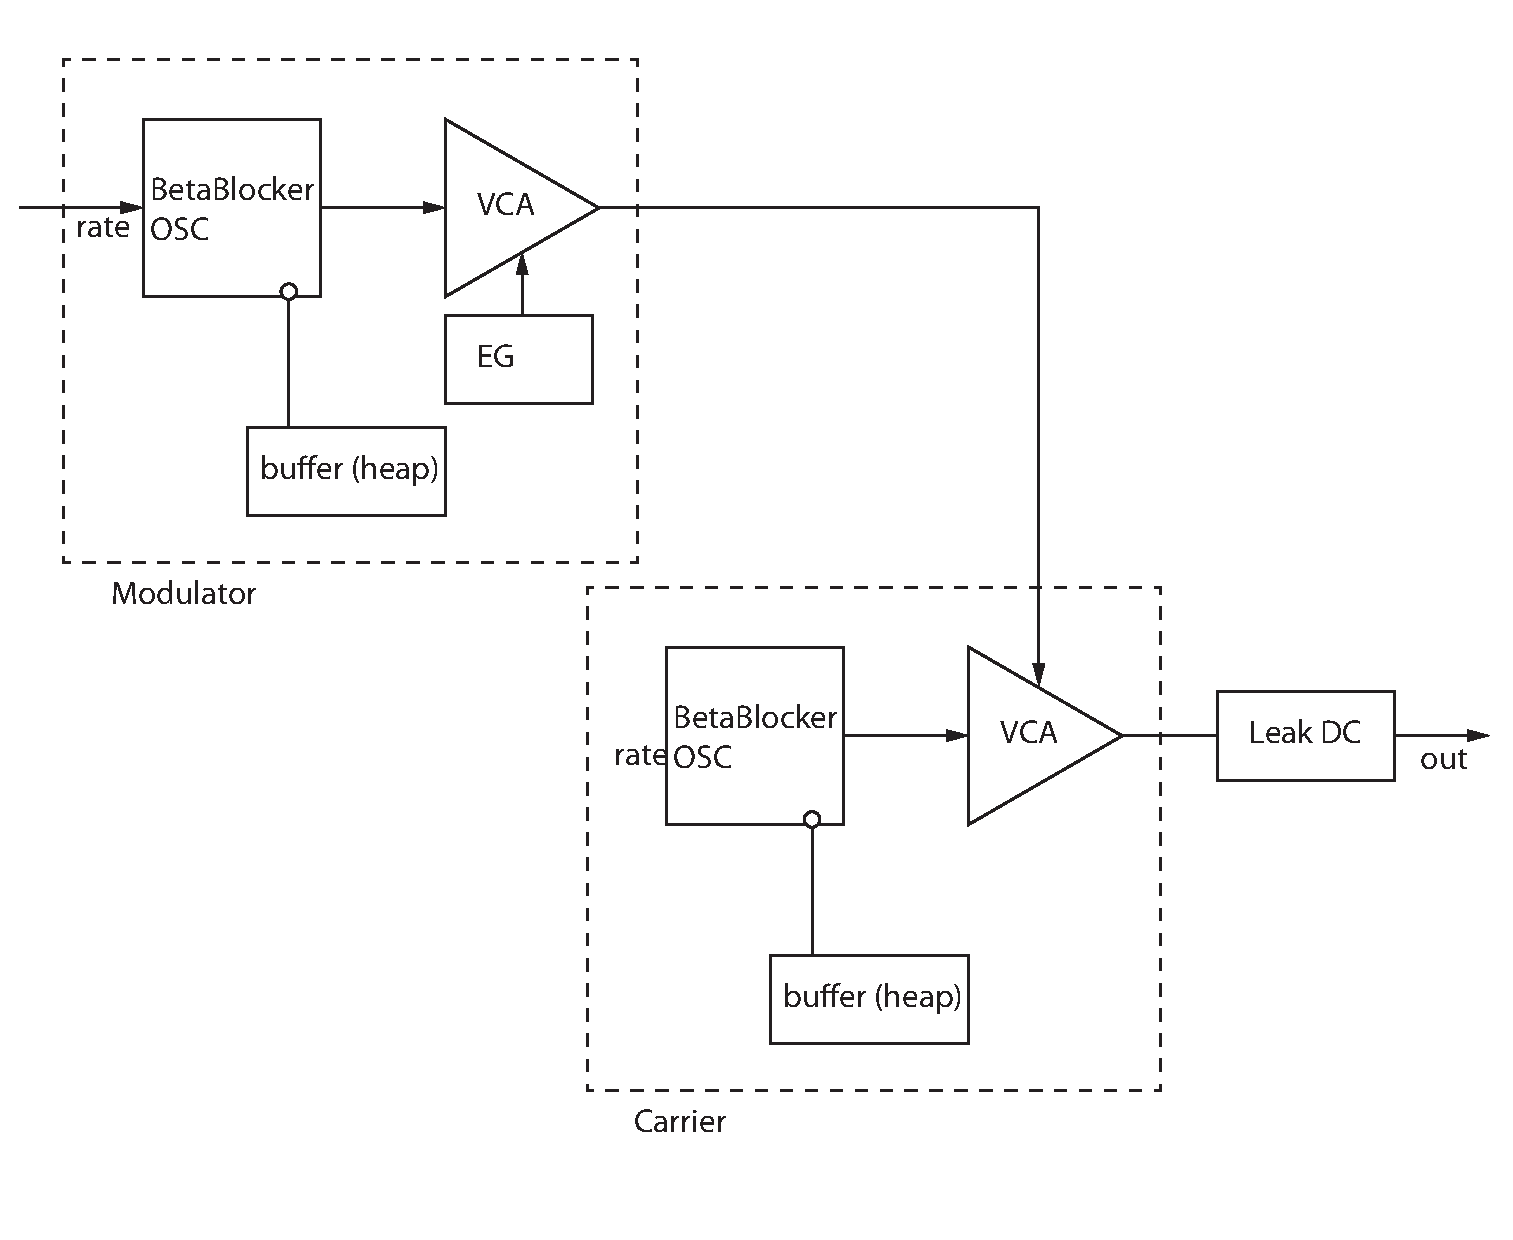
\includegraphics[height=3in]{AM-Betablocker}
% 	\caption{Amplitude modulation synthesis.}
% 	\label{fig:fig_AM-Betablocker}
% \end{figure}

\begin{figure}
	\centering
		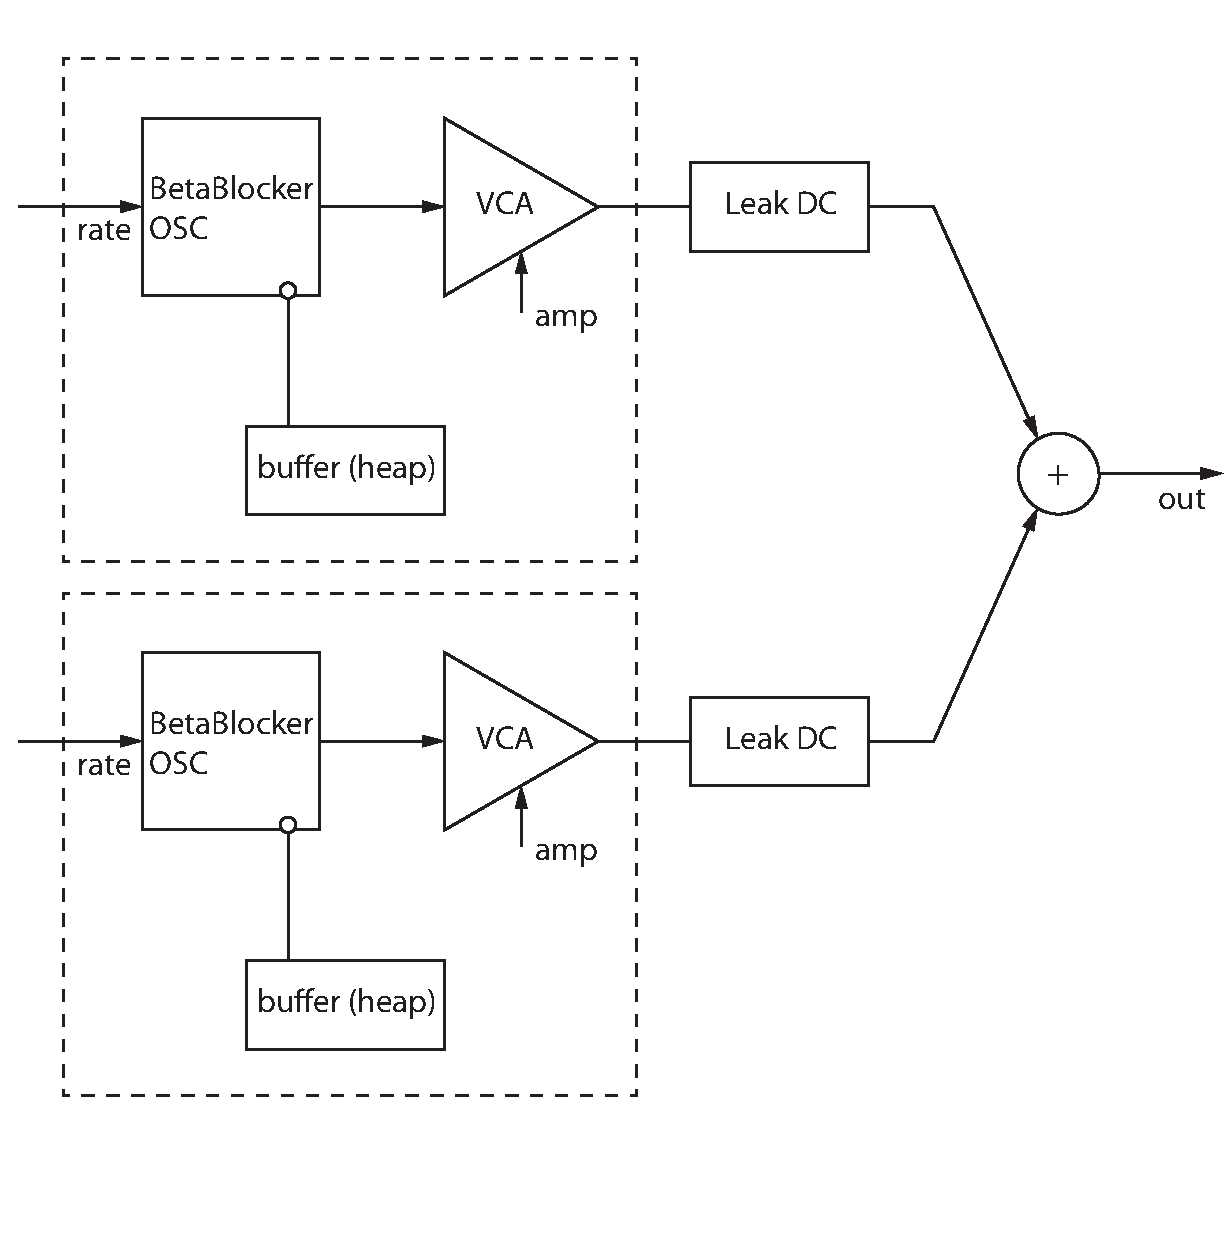
\includegraphics[height=4.5cm]{Additive-Betablocker}
		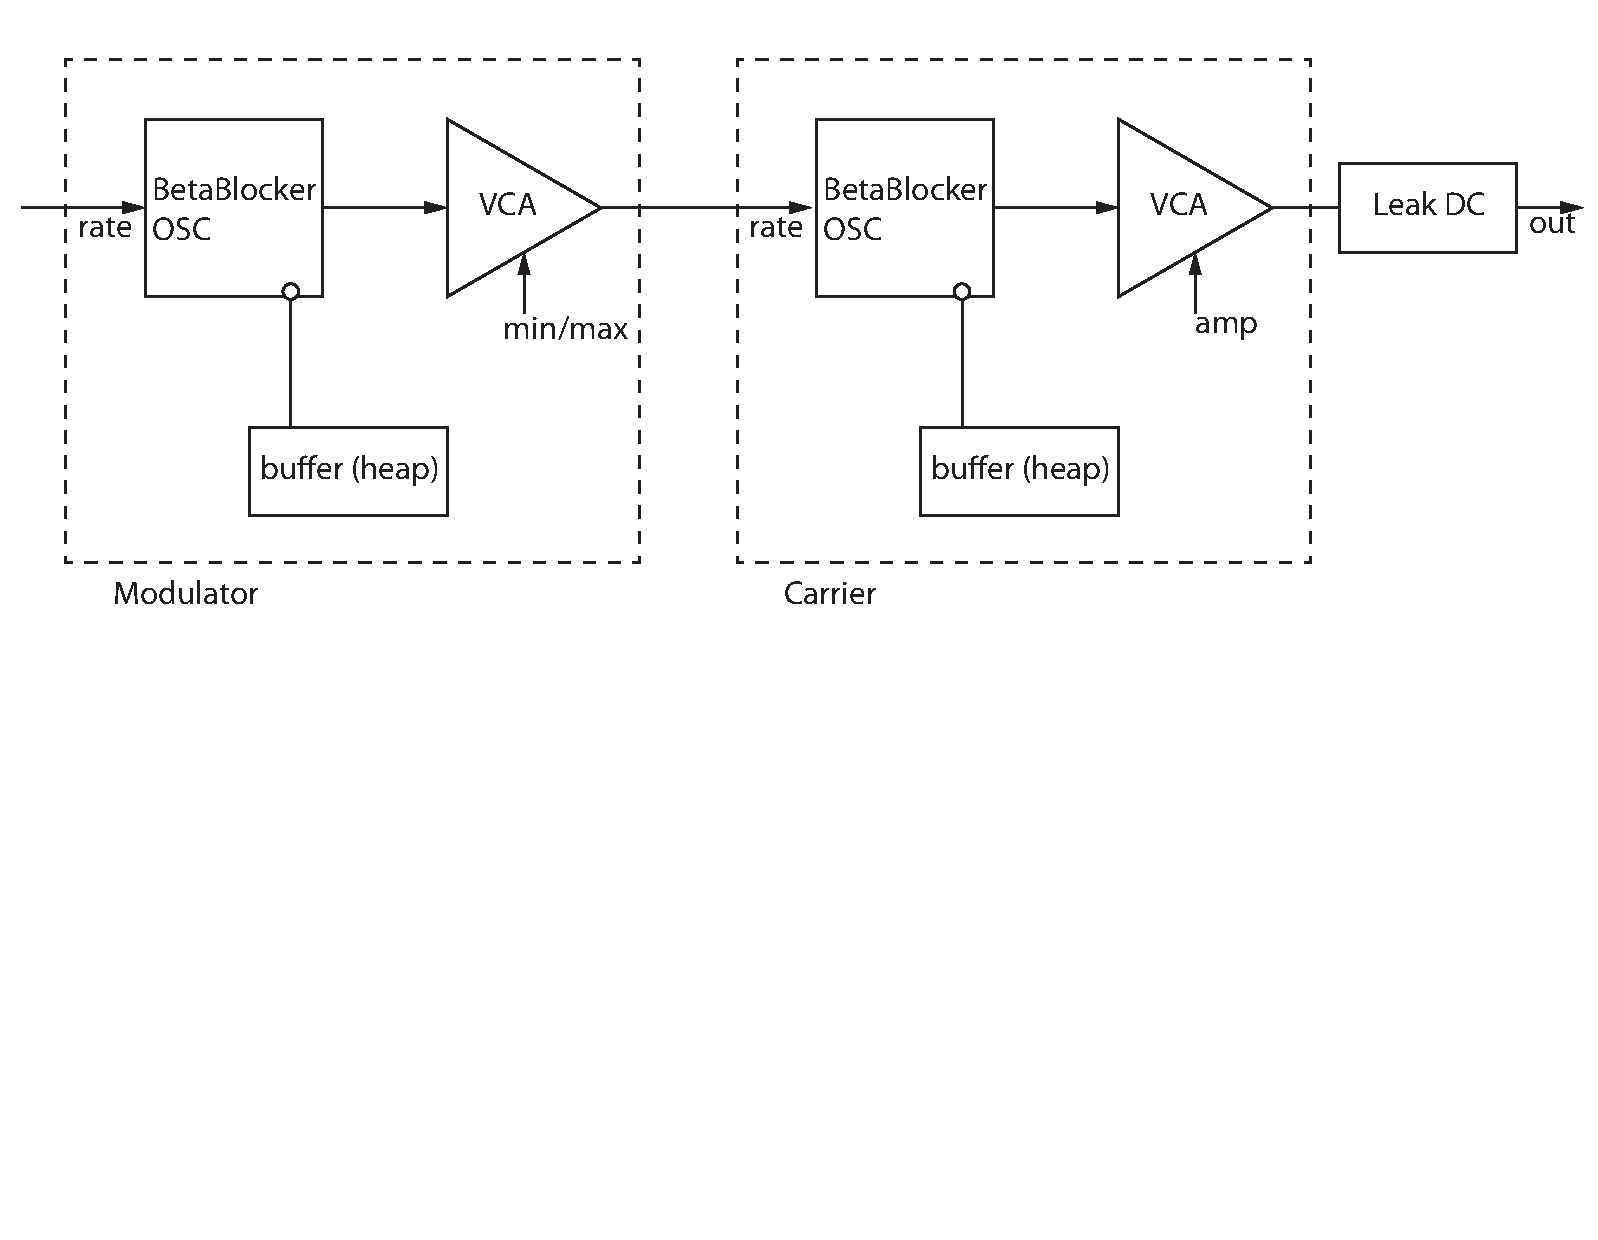
\includegraphics[height=4.5cm]{FM-Betablocker}
		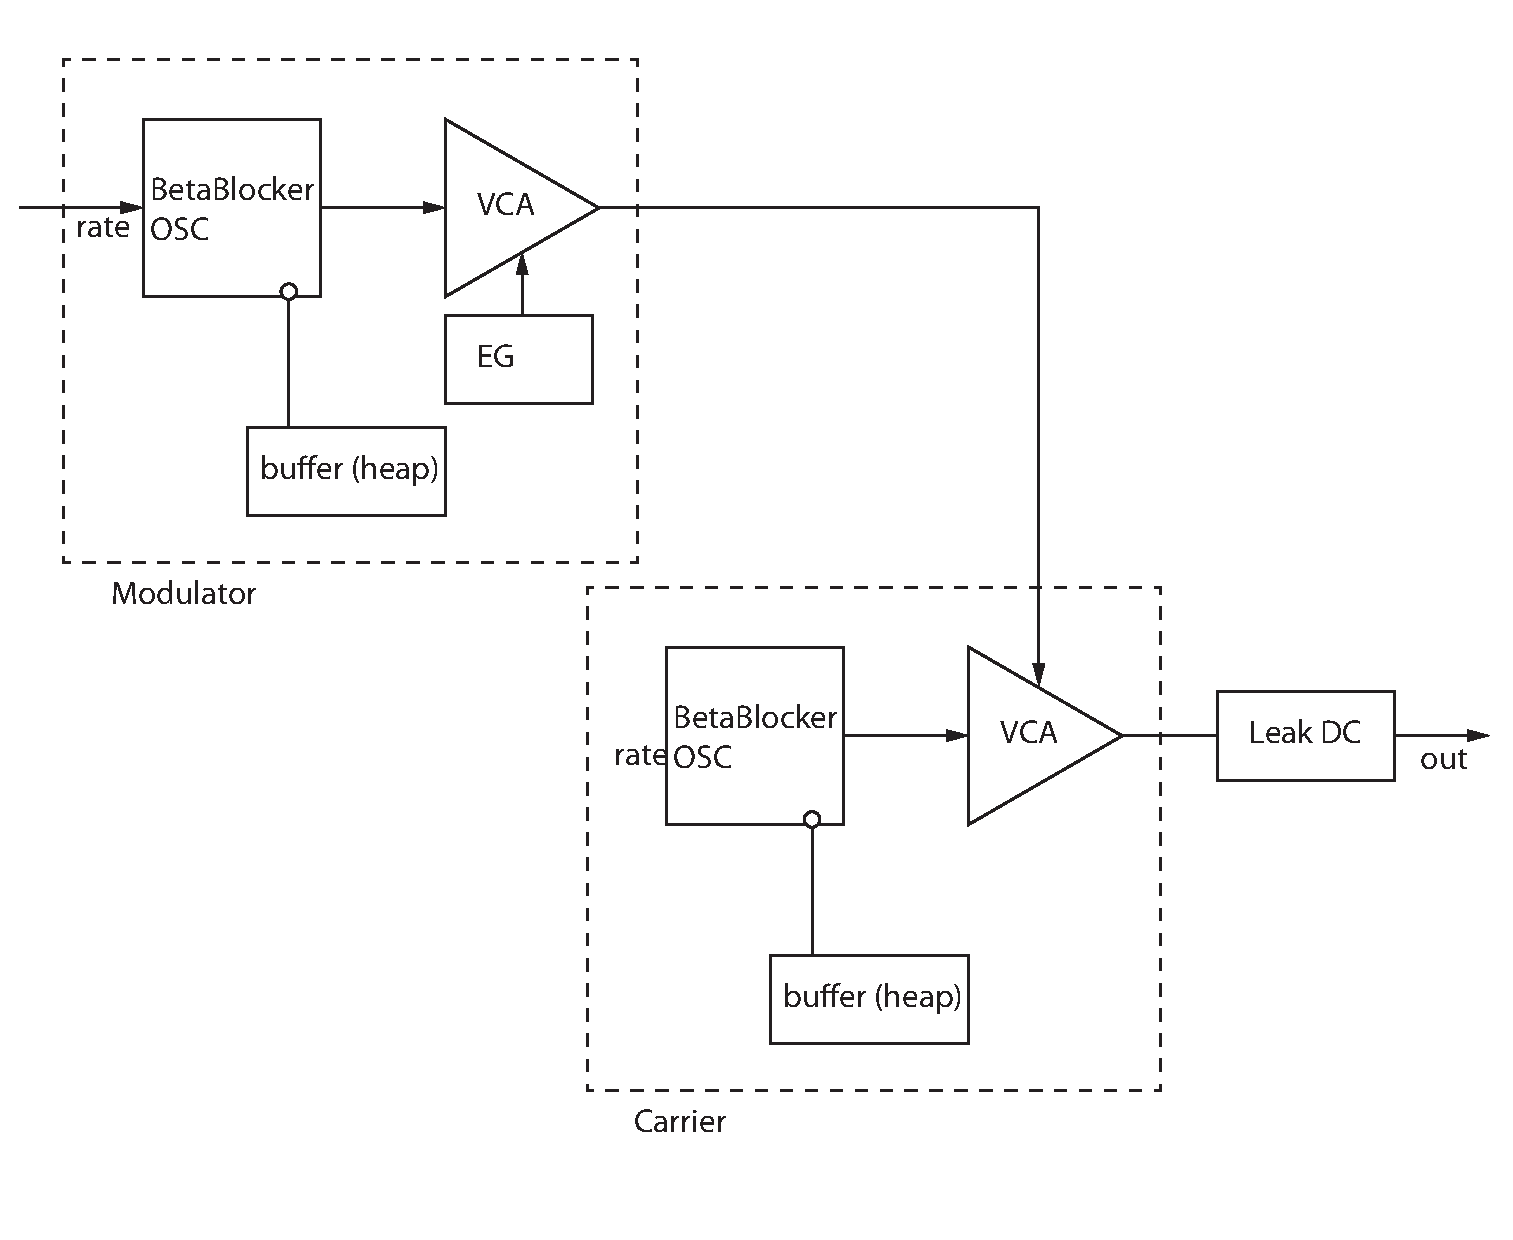
\includegraphics[height=4.5cm]{AM-Betablocker}
	\caption{Betablocker synthesis techniques.}
	\label{fig:fig_Additive-Betablocker}
\end{figure}

\begin{Verbatim}[fontfamily=courier, xleftmargin=\parindent]
{var output, pC, stack;

var numChains = 5;
var ctls = ['rates'.kr(1000!numChains), 'bufnums'.kr(0!numChains), 'amps'.kr(0.1!numChains)].flop;

output = ctls.collect{|ctl|
  # pC ... stack = BBlockerBuf.ar(
    ctl[0], ctl[1]
  );
  LeakDC.ar(stack[0] * ctl[2]);
};

Out.ar(0, output.sum)}.play;
\end{Verbatim}


FM:
\begin{Verbatim}[fontfamily=courier, xleftmargin=\parindent]
{var modulator, pC, stack, carrier;

modulator = Demand.ar(
  Impulse.ar('modRate'.kr(2000)), 
  'reset'.tr(0),
  DetaBlockerBuf('modBufnum'.kr(0))
).linlin(-1, 1, 'modMinAmp'.kr(200), 'modMaxAmp'.kr(1600));

# pC ... stack = BBlockerBuf.ar(
	modulator, 'carBufnum'.kr(0)
);
carrier = LeakDC.ar(stack[0]);

Out.ar(0, carrier)}.play;
\end{Verbatim}



AM:
\begin{Verbatim}[fontfamily=courier, xleftmargin=\parindent]
{var amp, pC, stack, output;

amp = Demand.ar(
  Impulse.ar('modRate'.kr(2000)), 
  'reset'.tr(0),
  DetaBlockerBuf('modBufnum'.kr(0))
).linlin(-1, 1, 'modMinAmp'.kr(200), 'modMaxAmp'.kr(1600));

# pC ... stack = BBlockerBuf.ar(
  'rate'.kr(1000), 'carBufnum'.kr(0)
);
output = LeakDC.ar(stack[0] * amp);

Out.ar(0, output)}.play;
\end{Verbatim}







\subsubsection{Genetic programming of sonic features} % (fold)
\label{sub:genetic_programming_of_sonic_features}


\subsection{Musical features} 
\label{sub:musical_features}

%%%%% on a rythmical level

% synthesis/human creation
%% programming sonic structures: e.g. drum pattern

\section{Betablocker and livecoding practice: a report} 
\label{sec:betablocker_and_livecoding_practice_a_report}

\subsection{Explicit livecoding vs. meta-livecoding} 
\label{sub:explicit_livecoding_}

% Explicit livecoding (here: on assembler level)
% meta-livecoding (here: the machine codes itself)


\subsection{Unfolding self modification to livecode pseudo-collaboration} 
\label{sec:unfolding_self_modification_to_livecode_collaboration}

Although the output of a given Betablocker stack is deterministic, it still is a mystery (i.e., not determinable) for the human mind - we want them to be like us so we suspend disbelief as a way to gain a tangible understanding

When working mostly with random data input, the pseudo-unpredicability kicks in quite heavily. 

At it's core, Betablocker provides a simple virtual machine for playing with music which is 'unstoppable' (any combination of instructions can be executed). It started off originally as a Fluxus scheme program, then got rewritten in C++ for the Nintendo DS, and has now been ported to Supercollider. I've built yet another Linux commandline version, and glued it to the Java Genetic Algorithms Package via Clojure.

This means I can continue with the genetic programming experiments and try evolving programs using a real genetic algorithm framework, using the betablocker instruction set. This is mainly just for kicks, but it's also partly to "grow" new strategies for livecoding betablocker and researching instruction sets more generally.
The first test was to try and find a program to just play note 99. I would write this in betablocker like this (using a text representation of the icon interface for convenience):

\begin{Verbatim}[fontfamily=courier, xleftmargin=\parindent]
   pshl 99 ; push the literal value 99 on to the stack
   note    ; play the top of the stack as a note 
\end{Verbatim}

First we need a fitness function to score the results from the programs which are generated:First we need a fitness function to score the results from the programs which are generated:

\begin{Verbatim}[fontfamily=courier, xleftmargin=\parindent]
(defn fitness [notes]
    (- 255 (Math/abs (- (first notes) 99))))
\end{Verbatim}

It takes a list of the notes played by a candidate program, and measures how far away the first element is from 99 - the bigger the number, the fitter the individual program is. I gave it 8 instructions to work with and a population of 500 individuals - after just a couple of generations, this chromosome/program popped up with a top fitness of 255 - meaning it was successfully playing note 99:

\begin{Verbatim}[fontfamily=courier, xleftmargin=\parindent]
99 46 213 89 7 142 23 168
\end{Verbatim}

Which when disassembled looks something like this:
\begin{Verbatim}[fontfamily=courier, xleftmargin=\parindent]
    99       ; <-- address 0 
    nop
    nop
    nop
    pshi 142 ; pushes contents of address at location 142 (which is 0)
    note     ; play the note
    nop
\end{Verbatim}

This program has grown taking advantage of the fact that the memory is initialised to zero, so if it dereferences a large address like 142 it will be zero and load the contents of the first byte - 99. It's this kind of wacked out approach genetic algorithms are great at finding/abusing.
The next problem, something a bit more general - create a sequence of notes which are all different to one another. The fitness function:

\begin{Verbatim}[fontfamily=courier, xleftmargin=\parindent]
(defn list-contains? [l i]
  (cond
   (empty? l) false
   (= (first l) i) true
   :else (recur (rest l) i)))

(defn fitness [a]
  (count
   (reduce
    (fn [r v]
      (if (not (list-contains? r v))
        (cons v r)
        r))
    '()
    a)))
\end{Verbatim}

This just counts the number of unique elements in the list - again, the higher the better. This one took longer, but eventually came up with this:  

\begin{Verbatim}[fontfamily=courier, xleftmargin=\parindent]
139 246 1 23 12 22 23 12 20 95 22 3
\end{Verbatim}

Which when disassembled:

\begin{Verbatim}[fontfamily=courier, xleftmargin=\parindent]
    nop
    nop
    org
start:
    note      ; play a note
    inc       ; increment top stack byte
    dup       ; duplicate top stack byte
    note      ; play a note (consumes 1 stack byte)
    inc       ; increment again
    pip 95    ; increment address 95 (junk - doesn't have any effect)
    dup       ; duplicate again
    jmp start ; return to the start
\end{Verbatim}

Which plays a rising sequence of notes, with none repeated, so the highest fitness achievable:

\begin{Verbatim}[fontfamily=courier, xleftmargin=\parindent]
0 1 2 3 4 5 6 7 8 9 10 11 12 13 14 15 16 17 18 19 20 21
\end{Verbatim}

This is already doing much better than the genetic programming I was mucking about with before - indeed there seems to be some literature on evolving java bytecode, but with betablocker there is an advantage that you don't need to enforce the correctness of the programs before they can be run.


Following on from the first BetaBlocker genetic algorithm bytecode experiments, in addition to the "most different notes" fitness function I added a similar calculation for the first derivative (ie. the difference between the notes in time order). This was an attempt to steer the evolution away from simple scales and into more complex patterns.

\begin{Verbatim}[fontfamily=courier, xleftmargin=\parindent]
(defn deriv [l]
  (cond
   (empty? l) '()
   (empty? (rest l)) '()
   :else (cons (- (first (rest l)) (first l))
               (deriv (rest l)))))
\end{Verbatim}
	       
The code to find the first derivative of a sequence of notes - eg. (deriv '(1 2 3 2 6 7)) => (1 1 -1 4 1). We then add this to the fitness function which looks like this:

\begin{Verbatim}[fontfamily=courier, xleftmargin=\parindent]
(+ (count (num-unique res)) ; unique notes are good
   (count (num-unique (deriv res))) ; unique gaps between notes are good
   (min (count res) 20)) ; lots of notes are good (stop at 20)
\end{Verbatim}
   
This resulted in the following bytecode to emerge from the primordial soup: 23 17 7 6 23 21 9 23 8 212 3 2 4 2 180 124 - which disassembles to:

\begin{Verbatim}[fontfamily=courier, xleftmargin=\parindent]
	note      ; stack is empty, so plays zero
	not       ; pushes bitwise "not" of zero => 255
loop:
	pshi 6    ; push the contents of address 6 (-> 9 = 212)
	note      ; play the note (212)
	pdp 9     ; decrement address 9 (212 becomes 211)
	note      ; plays 255 first time, 0 after that when stack is empty
	pop 212   ; stack is now empty so writes 0 to adress 212
	jmp loop  ; goto loop
	jmpz 2    ; junk, we never reach here
	nop
	nop
\end{Verbatim}

The arrows show the indirection which helps as this one is a bit tricky to pull apart. It's the first time I've seen self modification emerge - it decrements the "212" and uses it as a variable for the note sequence. Combining the pshi and pdp like this is a nice trick I can make use of when programming betablocker myself.
The program is self destructive - the "pop" which otherwise does nothing of use will eventually write zeros over the program itself if it's run for a few more cycles than the 100 I'm testing the programs for.
The output looks like this: 

\begin{Verbatim}[fontfamily=courier, xleftmargin=\parindent]
0 212 255 211 0 210 0 209 0 208 0 207 0 206 0 205 0 204 0 203 0 202 0 201 0 200 0 199 0 198 0 197 0 196
\end{Verbatim}

According to our fitness function, the interleaved zeros give it a very high scoring derivative list:

\begin{Verbatim}[fontfamily=courier, xleftmargin=\parindent]
212 43 -44 -211 210 -210 209 -209 208 -208 207 -207 206 -206 205 -205 204 -204 203 -203 202 -202 201 -201 200 -200 199 -199 198 -198 197 -197 196
\end{Verbatim}

However the actual pattern is not so interesting, so still more work needed on the fitness criteria.

For the next attempt in BetaBlocker bytecode evolution I wanted to favour patterns that had a rhythmic nature by measuring them with this function:

\begin{Verbatim}[fontfamily=courier, xleftmargin=\parindent]
(defn freq [l n]
  (defn _ [c]
    (cond
     (>= (+ c n) (count l)) 0
     (= (nth l c) (nth l (+ c n))) (+ 1 (_ (+ c 1)))
     :else (_ (+ c 1))))
  (_ 0))
\end{Verbatim}

Which looks for repeating values spaced apart by "n" positions, so (freq '(100 1 2 3 100 4 5 6 100 7 8 9 100) 4) returns 3, as it finds 3 pairs of equal values (100) distanced by the specified 4 positions.
With this fitness function:

\begin{Verbatim}[fontfamily=courier, xleftmargin=\parindent]
(+ (* 50 (count (num-unique res))) ; unique notes are very good
   (freq res 4) ; equal notes every 4 beats are good
   (freq res 6)) ; equal notes every 6 beats are good
\end{Verbatim}

We favour rhythmic components of 4 or 6 beats and boost the uniqueness score by multiplying it by 50. After some generations, we get a high scoring individual: 23 23 13 22 7 12 17 20 12 23 23 5 0 7 12 3 
Which disassembles as:

\begin{Verbatim}[fontfamily=courier, xleftmargin=\parindent]
loop:
    note    ; play & remove top of stack (zero when empty)
    note    ; play & remove top of stack
    dec     ; decrement top of stack
    dup     ; duplicate - pushes a copy of stack top 
    pshi 12 ; push the value pointed at by address at 12 (self read)
    not     ; performs bitwise not on stack top
    pip 12  ; increment value at address 12
    note    ; play & remove top of stack
    note    ; play & remove top of stack
    pshl 0  ; pushes this literal number (the 0 is at address 12)
    pshi 12 ; push the value pointed at by 12 (self read)
    jmp loop
\end{Verbatim}
    
This program creates a pattern from 4 separate sources, using all 16 bytes of code:


The result: "0 0 232 255 23 1 232 254 13 2 242 253 22 3 233 252 7 4 248 251 12 5 243 250 17 6 238 249 20 7 235 248 12 8" scores poorly for it's rhythmic patterns, but it's probable that this surprising local maxima was found by the early influence of the rhythmic fitness criteria on it's ancestor populations. 

\subsection{Embedded evolved code} 
\label{sub:embedded}

A system for creating an abundance of useless software for tiny devices. Spork Factory evolves programs that run on Atmel processors \u2013 the same make as found on the Arduino, in this case the ATtiny85 \u2013 a �2.50 8 pin 8bit CPU. I\u2019m currently simply using a piezo speaker as an output and evolving programs based on the frequency of the sound produced by flipping the pins up and down, so creating 2bit synths using the Fourier transform as the fitness function. With more hardware (input as well as output) perhaps we could evolve small robots, or even maybe cheap claytronics or programmable matter experiments.

This project reuses the previous genetic programming experiments (including jgap as its genetic algorithm framework), and is also inspired by Till Bovermann's recent work with Betablocker in Supercollider for bytecode synthesis.

The programs generated don't use the Atmel instruction set directly, but interpret a custom one derived from Betablocker for two reasons. Atmel processors separate their instruction memory from data (the Harvard architecture) which makes it difficult to modify code as it's running (either uploading new evolved code or running self modifying instructions), the other is that using a simplified custom instruction set makes it easier for genetic algorithms to create all kinds of strange programs that will always run.

I've added an 'OUT' instruction, which pops the top of the stack and writes it to the pins on the ATtiny, so the first thing a program needs to do is generate and output some data. The second thing it needs to do is create an oscillator to create a tone, after that the fitness function grades the program on the amount of frequencies present in the sound, encouraging it to make richer noises.

Here are two example programs from a single run, first the ancestor, a simple oscillator which evolved after 4 or 5 generations:

\begin{Verbatim}[fontfamily=courier, xleftmargin=\parindent]
    out
    out
    nop
    nop
    dec
    nop
    nop
    nop
    out
    nop
    jmpz 254
    nop
    nop
    nop
    dup
\end{Verbatim}

It's simply outputting 0's, then using the 'dec' to decrement the top of the stack to make a 255 which sets the rightmost bit to 1 (the one the speaker is attached to) and then loops with the 'jmpz' causing it to oscillate. This program produces this fft plot:

\begin{figure}
	\centering
		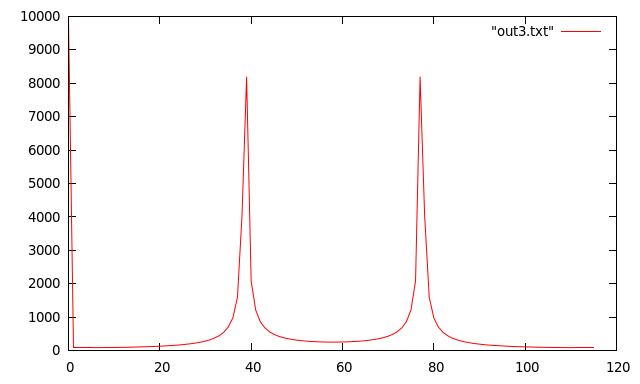
\includegraphics[width=13cm]{spork1}
	\caption{XOR rave}
	\label{fig:fig_spork1}
\end{figure}

After 100 or so further generations, this descendant program emerges. The dec is replaced by \u2018pshl 81\u2032 which does the same job (pushes the literal value 81 onto the stack, setting our speaker bit to 1) but also uses a \u2018dup\u2019 (duplicate top of the stack) to shuffle the values around to make a more complex output signal with more frequencies present:

\begin{Verbatim}[fontfamily=courier, xleftmargin=\parindent]
loop:
    out
    out
    not
    nop
    pshl 81
    pshi 149
    out
    nop
    out
    nop
    dup
    psh 170
    jmp loop
\end{Verbatim}

\begin{figure}
	\centering
		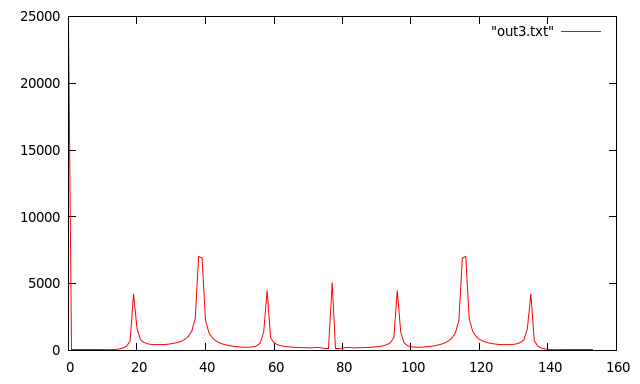
\includegraphics[width=13cm]{spork2}
	\caption{XOR rave}
	\label{fig:fig_spork2}
\end{figure}

Also robotics, an evolved light follower:

\begin{Verbatim}[fontfamily=courier, xleftmargin=\parindent]
    pshl 171 
loop:
    lmot 
    leye 
    pip 111 
    pip 30 
    rmot 
    reye 
    pshl 214 
    nop 
    lmot 
    jmp loop
\end{Verbatim}

\begin{figure}
	\centering
		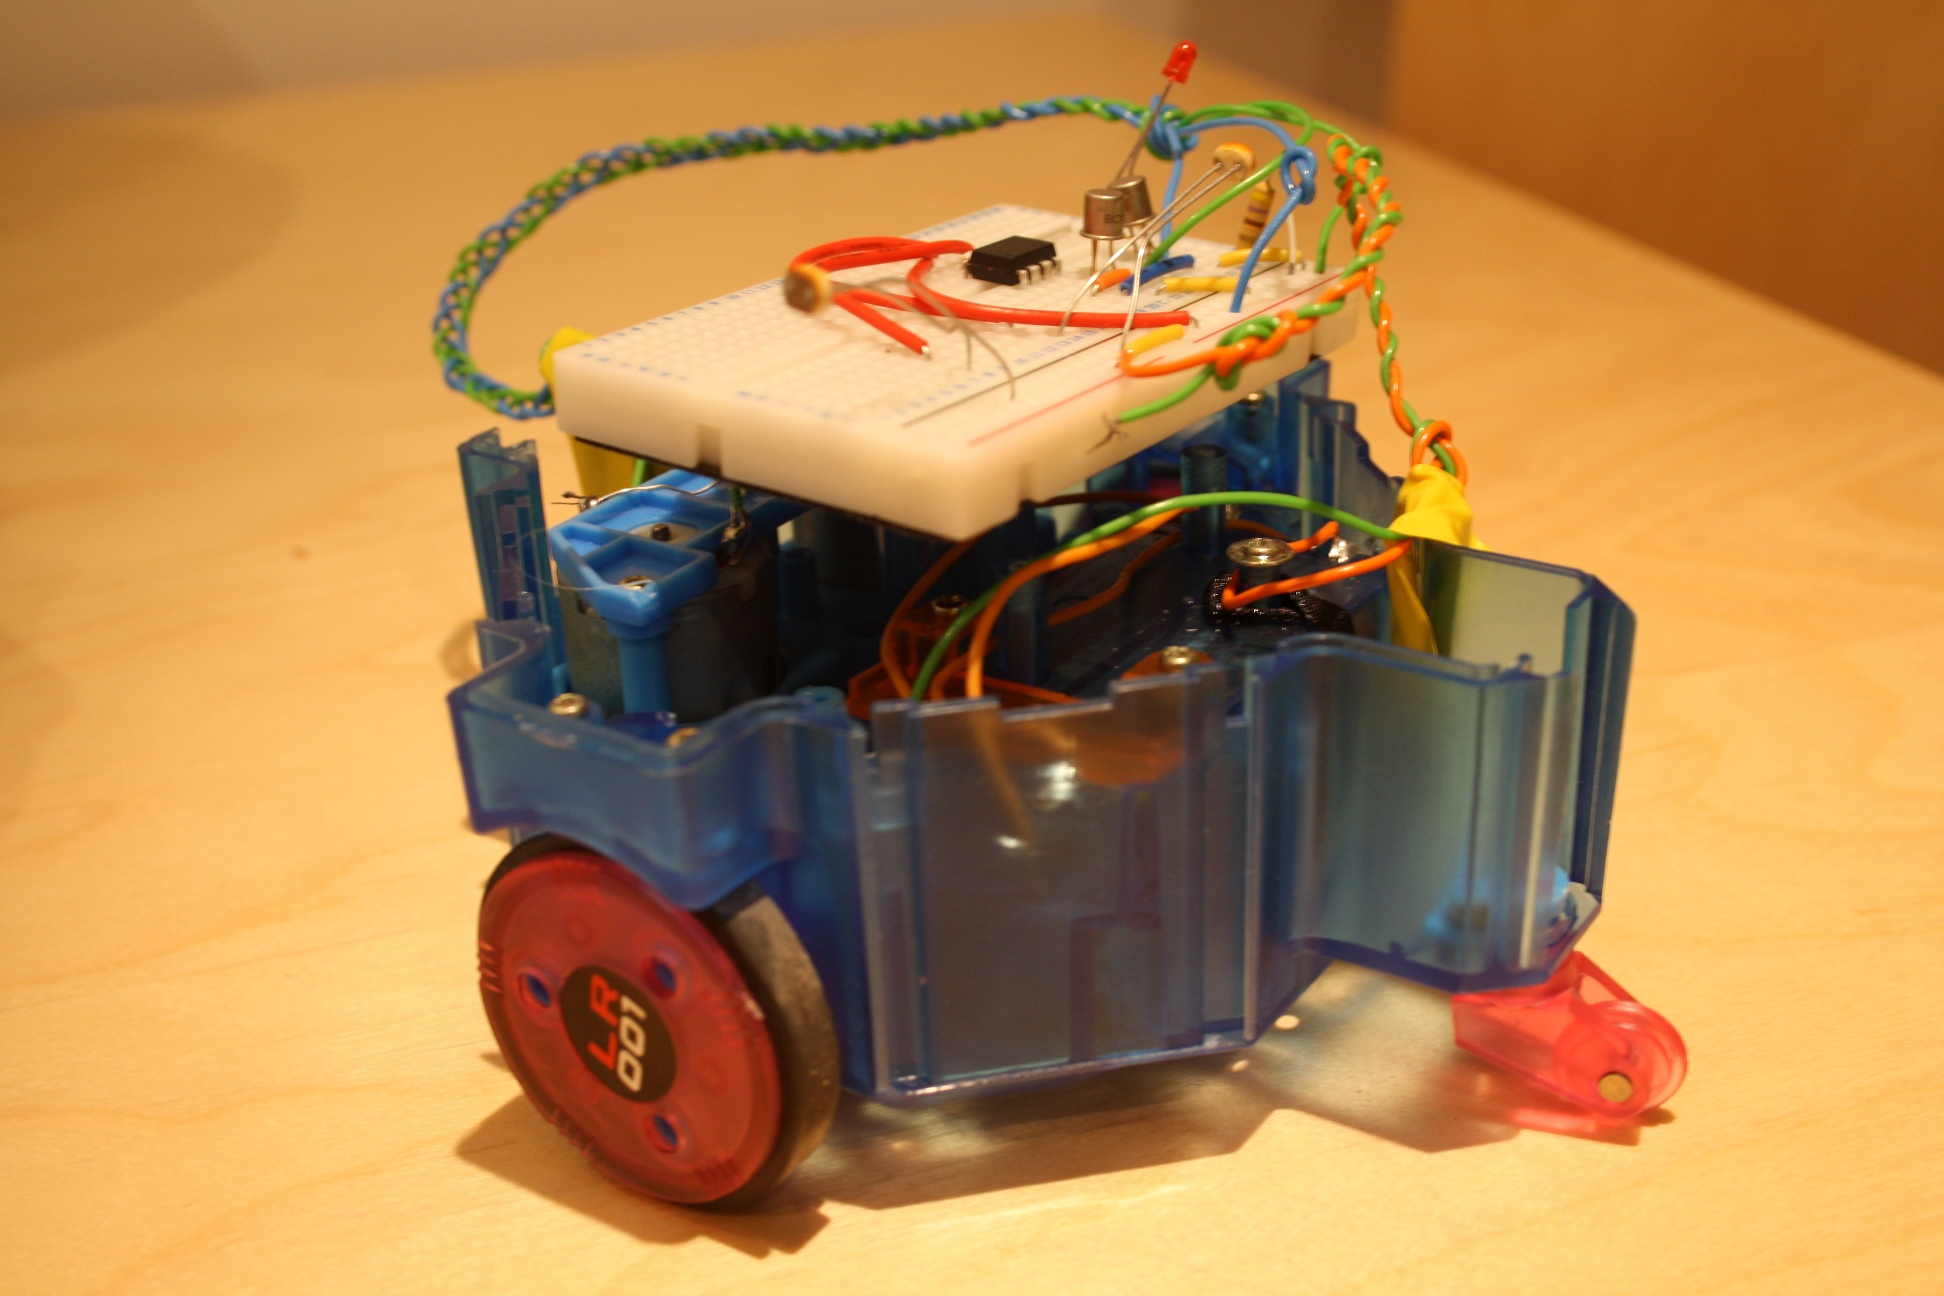
\includegraphics[width=13cm]{bbbot}
	\caption{caption}
	\label{fig:fig_bbbot}
\end{figure}

\subsection{Towards Amorphous livecoding} 
\label{sub:amorphous_livecoding}

\begin{figure}
	\centering
		
\includegraphics[width=13cm]{amorphous}
	\caption{500 betablocker CPUs}
	\label{fig:amorphous}
\end{figure}

Departing in a new direction after evolved light follower robots, take 500 processor cores spread out in space. Give them a simple instruction set which includes a instruction to copy (DMA) 8 bytes of their code/data to nearby cores (with an error rate of 0.5%). Fill the cores with random junk and set them running. If we graph the bandwidth used (the amount of data transmitted per cycle by the whole system) we get a plot like this:
\begin{figure}
	\centering
		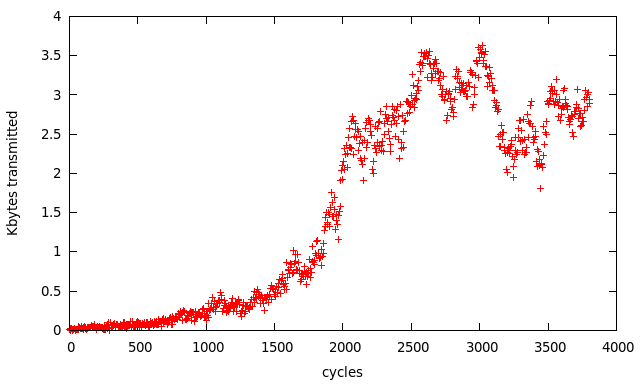
\includegraphics[width=13cm]{amorphous-bandwidth}
	\caption{Bandwidth}
	\label{fig:amorphous-bandwidth}
\end{figure}

This explosion in bandwidth use is due to implicit emergence of programs which replicate themselves. There is no fitness function, it's not a genetic algorithm and there is no guided convergence to a single solution - no 'telling it what to do'. Programs may arise that cooperate with each other or may exhibit parasitic behaviour as in alife experiments like Tierra, and this could be seen as a kind of self modifying, emergent Amorphous computing - and eventually, perhaps a way of evolving programs in parallel on cheap attiny processor hardware.


% pseudo-interaction
%% human (behaviour) <---> computer (pseudo-proactive behaviour)

% a turing-test for livecode companions

\subsection{Betablocker livecoding practice}
\label{sub:livecoding_performance_practice_influenced_by_betablocker}

% \subsubsection{Dave's Betablocker practice}
% \label{sub:daves_performance_style}
% 
% 
% \subsubsection{Till's Betablocker practice}
% \label{sub:tills_performance_style}

Subsequent, we describe Betablocker-based performances in their order of appearance.

\subsubsection{SuperCollider symposium London -- livecoding and visuals [4.2012]}
\label{sub:livecoding_and_visuals}

For the livecoding gig at the SuperCollider Symposium 2012, London, the two authors performed together for the first time. 
As they lived at that time already in different countries, they developed a remote rehearsal routine, i.e. each of them prepared his part as a sound recording and the other performed on top of it.

At the same time, both authors prepared their life sets.

Till's aesthetic goal for the performance was to play poly-rhythmical layers of coloured, noisy sounds with a setup purely based around his SuperCollider Betablocker implementation. 
At the same time, he aimed for a certain amount of transparency, i.e., it should be possible to not only see the changes he is making to the code but also how  Betablocker engines alter the heaps' content.
This meant 
(a) to develop a visual representation of the heaps he was playing, 
(b) to design a textual helper environment for his livecoding, mainly providing text blocks, and
(c) to pre-select heaps that he used as "raw materials" for his part of the  performance.

%%% a visual language
different approaches to visual patterning (8bit display, scopes and buffer-iris)


\begin{figure}
	\centering
		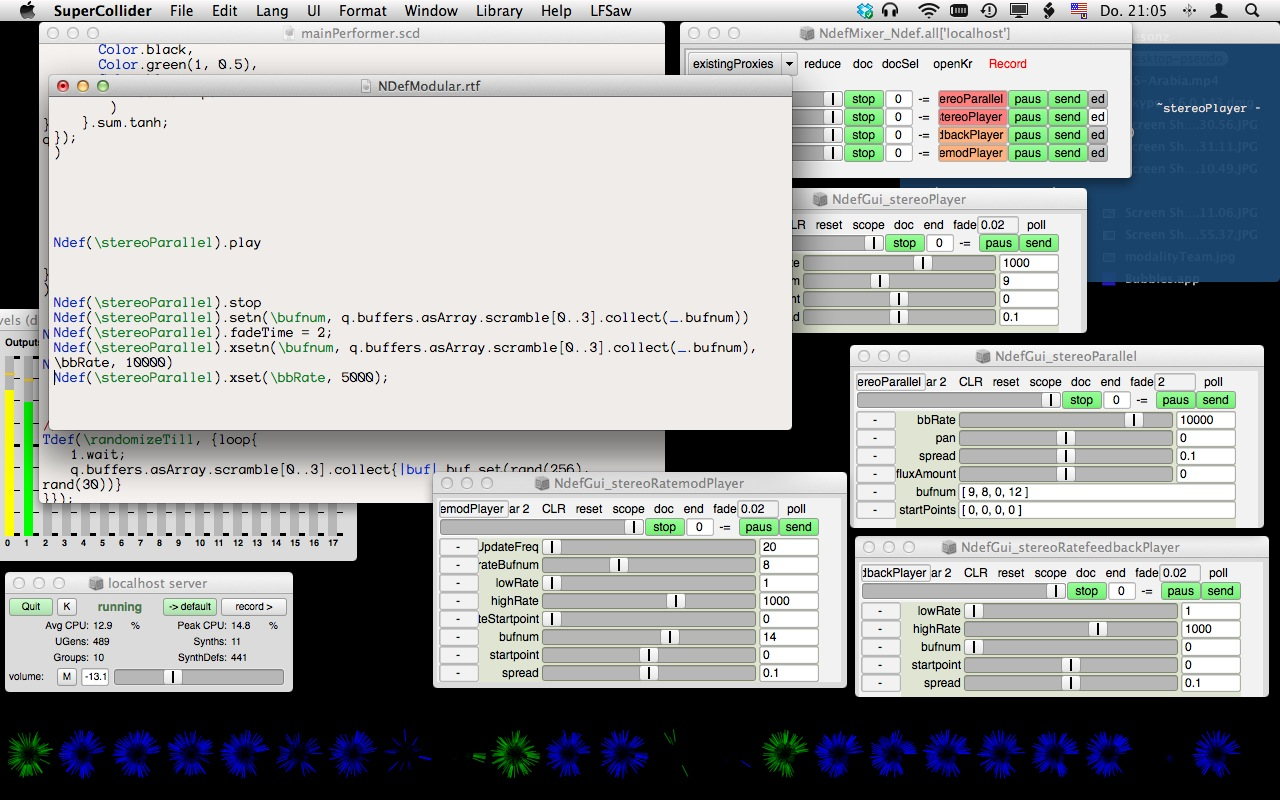
\includegraphics[width=13cm]{2012-SuperColliderSymposiumLiveCodingEnvironment-till}
	\caption{Till's livecoding environment as used at the SuperCollider symposium 2012, London.}
	\label{fig:fig_2012-SuperColliderSymposiumLiveCodingEnvironment-till}
\end{figure}


\begin{figure}
	\centering
		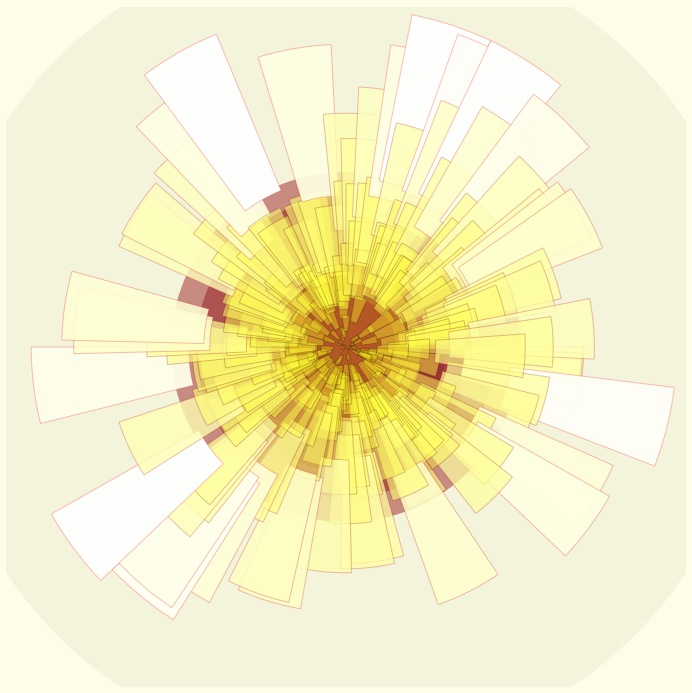
\includegraphics[width=6cm, height=6cm]{2013-heapIris-white}
		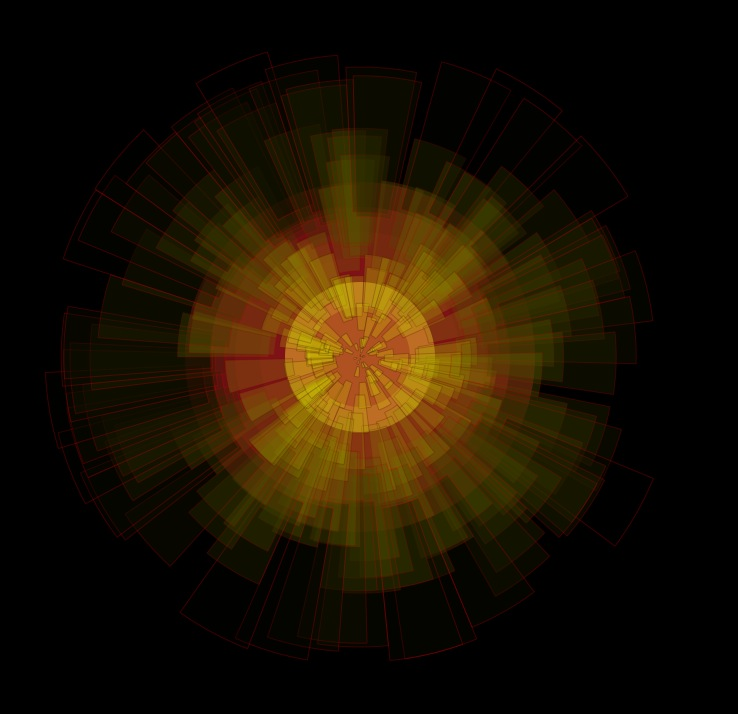
\includegraphics[width=6cm, height=6cm]{2013-heapIris-black}
	\caption{Iris-style visualisations of heaps.}
	\label{fig:fig_2013-heapIris-white}
\end{figure}

% \begin{figure}
% 	\centering
% 		
\includegraphics[width=2in]{binaryRepresentation-01}
% 		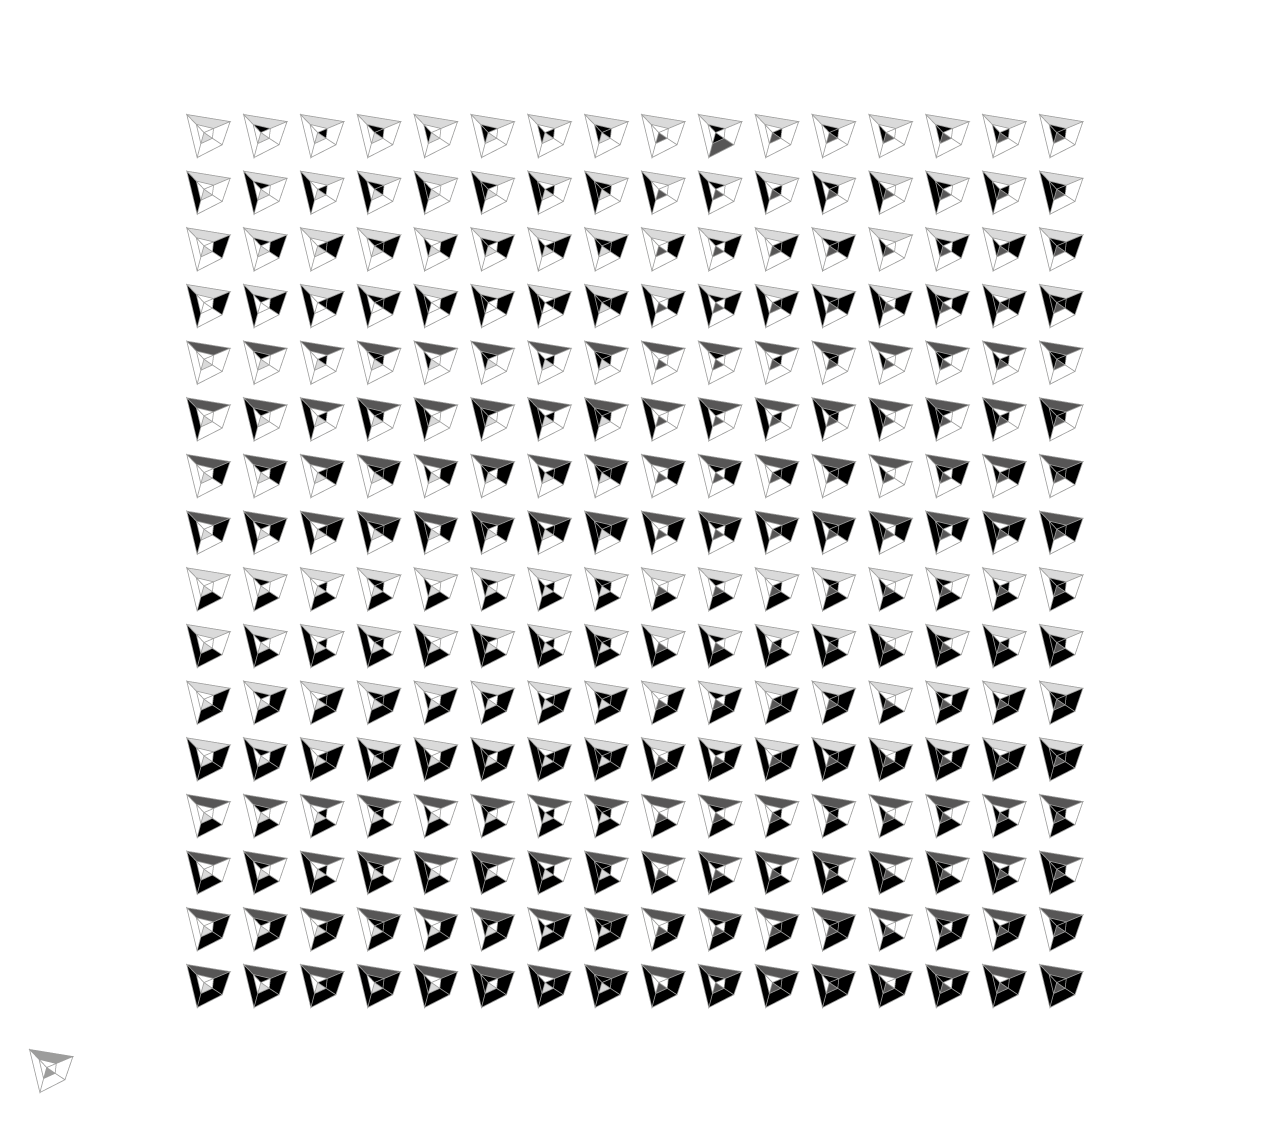
\includegraphics[width=2in]{binaryRepresentation-02}
% 		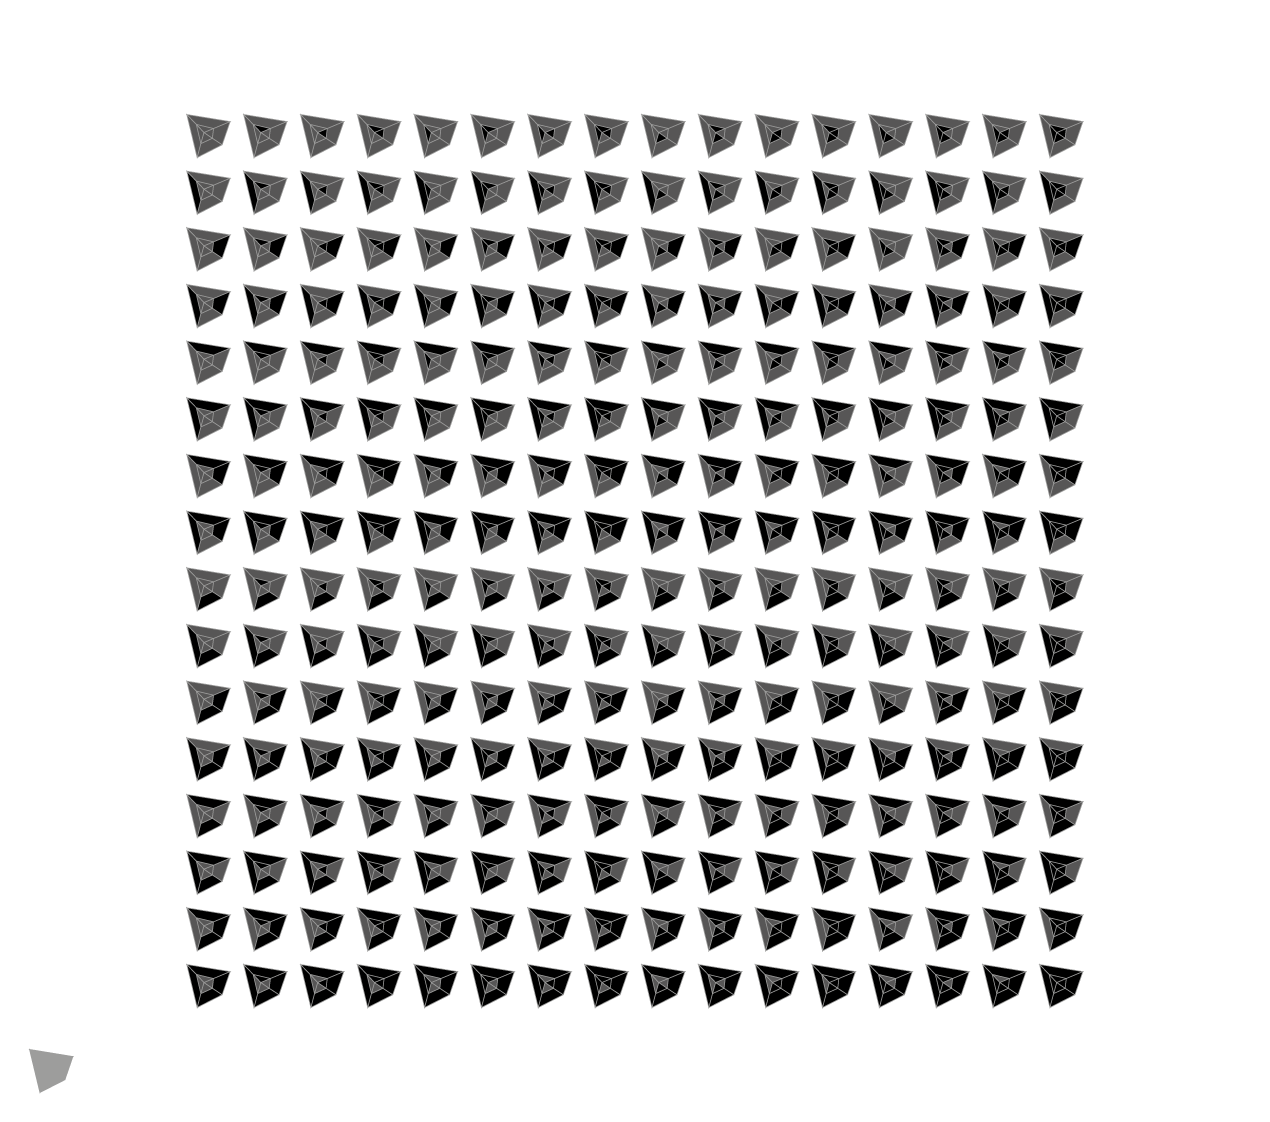
\includegraphics[width=2in]{binaryRepresentation-03}
% 	\caption{Visual representation of 2x8-bit.}
% 	\label{fig:fig_2013-heapIris-white}
% \end{figure}


\subsubsection{Oulipop -- translation of codes [5.2012]}
\label{sub:oulipop}
2 Performers, 1 laptop, 20 minutes. Till Bovermann and Sara Hildebrand Marques Lopes.

%%% translation of codes: Oulipop
Relation between written text, code and sound.

Manipulating texts according to Oulipo rules (\cite{mathews2005-oul}).
Meta-level live-coding. 
Each keystroke triggers a process that translates the current text's characters into a set of commands for a fictional CPU. 
Treated as a sound signal, the ever-changing output of that CPU is played back, and thereby influences the performers' decisions on how to further alter the text. 
Over the course of the performance, an initially meaningful text turns into nonsense before it eventually settles into a new and often surprising semantical meaning.\footnote{For more information and a documentation video, see \url{http://www.tai-studio.org/oulipop/}.}
\begin{figure}
	\centering
		\includegraphics[width=13cm]{20120509-IMG_3278}
	\caption{The Oulipop performance environment.}
	\label{fig:fig_20120509-IMG_3278}
\end{figure}


\section{Research in computing processes (Till's junkyard)}
\label{sub:research_in_computing_processes}

Based on phenomenological methods/maxims, treating the subject of investigation (here: BetaBlocker) as being only perceivable \emph{through} phenomena (things "present to the mind"). 
As we are interested in sonic qualities, the selected modality of the observed phenomena are mainly of sonic nature.
On our way through the system, though, other introspective as well as extrospective data emerged and was taken into account.

To illustrate the research journey, we will now list key events that happened:

Starting point was a collection of C files that defined the BetaBlocker core.
To keep things simple at the beginning, a crucial strategy in implementations, we decided to fill the heap with a very simple program resembling a sawtooth \texttt{[ORG, INC, JMP, 0]}. 
After successfully listening to this basic setup, we replaced the hardcoded heap with one that gets initialised with random values between $0$ and $255$.\footnote{\url{http://tai-studio.org/index.php/2011/05/betablocker-ugen/}}


Airy, sustained sound clouds; mostly high-pitched broken up occasionally by a rhythmical pattern


\begin{itemize}	 
\item Implemented access to heap's data. This means that it can be set, read and manipulated while running. Also, several engines can share a heap. 
	% http://tai-studio.org/index.php/2011/08/detablockerbuf-8channel/ 
\item helper classes facilitating the generation of BBlocker programs 
	% http://tai-studio.org/index.php/2011/08/twentydblockers/ 
\item further sonic exploration, listening sessions 
	% http://tai-studio.org/index.php/2011/10/betablocker-pieces/

	For now, the layout is always additive, i.e., several BBlocker engines next to each other

\item Idea generation
	% http://tai-studio.org/index.php/2011/10/betablocker-theory-day/ 
\item Visual representation
	% http://tai-studio.org/index.php/2011/11/attempt-for-representing-2x8bit/
\item public demo video
	% http://tai-studio.org/index.php/2011/12/dblockerintro/ 
\item adding convenience methods play/scope/plot to BBlockerProgram based on feedback of first introduction to a non-programmer
	% http://tai-studio.org/index.php/2011/12/cambridge-day-4/ 
\item New iteration of the BetaBlocker wrapper, adding more output (pos and whole stack) and removing the possibility to control it with demand rate,
	% http://tai-studio.org/index.php/2011/12/60-panned/ 
	includes a sound study.
\item Multi-out UGen with audio-rate input
	% http://tai-studio.org/index.php/2011/12/cambridge-day-8/
\item Decision to focus on sonic aspects. Therefore tried to write/design programs with specific sonic features in mind.
	% http://tai-studio.org/index.php/2011/12/cambridge-days-912/
\item FM-like synthesis strategy added
\item Performance at Cambridge, fixed setup
\item Rehearsal for SuperCollider Symposium
\item Concert at SuperCollider Symposium
\item Workshop at UdK.
\item Oulipop performance
\end{itemize}



\section{Meta}
\label{sec:meta}




\vspace*{24pt}





\vspace*{24pt}


% % format for Heading-B style
% \subsection{Format for Heading-B Style; Use This for Subsection Headings}
% 
% Insert body text here.  
% 
% % format for Heading-C style
% \subsubsection{Format for Heading-C Style; Use This for Minor Sub-subsection Headings}
% 
% Insert body text here.
% 
% In the initial manuscript submission, you are encouraged to include figures (with captions) inline with the text, for ease of reading during the review process. For example, like this:
% 
% % include figures in text with captions for initial submission, like this:
% \begin{figure}[htpb]
% \begin{center}
% \includegraphics{myFigure.pdf}
% \caption{Insert Figure caption here.}
% \label{fig:myFigure}
% \end{center}
% \end{figure}
% 
% However, for the final version after the manuscript has been accepted, all figures should be moved to the end so that the text only contain markers like ``[Figure 1 about here]'' near where the figure would normally have occurred. You can rearrange the text to this effect simply by enabling the package {\tt endfloat} as suggested in the header of this document.
% 
% 
% % equations
% You can insert equations inline with the text like this:
% 
% \begin{equation}
% 	\label{radupdate}
% 		\Psi_{N}^{n+1} = m_{N}^{(-)}\Psi_{N-1}^{n}+m_{N}^{(0)}\Psi_{N}^{n} + q_{N}\Psi_{N}^{n-1}
% \end{equation}
% where
% \begin{eqnarray*}
% 	m_{N}^{(-)} &=& \frac{\lambda^2}{2\tau}\left(S_{N+1}+2S_{N}+S_{N-1}\right)\\
% 	m_{N}^{(0)} &=& \frac{1}{\tau}\left(2-\frac{\lambda^2}{2}\left(S_{N+1}+2S_{N}+S_{N-1}\right)\right)\\
% 	q_{N} &=& \frac{1}{\tau}\left(\frac{\gamma^2 k^2}{2h}\left(S_{N+1}+S_{N}\right)\left(\frac{\alpha_{1}}{k}-	\alpha_{2}\right)-1\right)
% \end{eqnarray*}
% and where 
% \begin{equation*}
% 	\tau = \frac{\gamma^2 k^2}{2h}\left(S_{N+1}+S_{N}\right)\left(\frac{\alpha_{1}}{k}+\alpha_{2}\right)+1
% \end{equation*}
% 
% % Use this environment for inserting source code examples.
% % Note, that this will print out text in the document exactly as you type it here in the .tex file. That means you can add empty spaces, tabs, blank lines here and they will be printed out like this in the document.). 
% %For more information check out the LaTeX-Package 'fancyvbr' documentation
% %
% \begin{Verbatim}[fontfamily=courier, xleftmargin=\parindent]
% Use this style for program code, for example:
% main() {
%     printf("Hello World\n");    
% }
% \end{Verbatim}
% 
% %use of references
% Some examples for the use of references in the text:\\
% %author name in sentence, single authors
% \cite{Ano08}, \cite{Bele68}, \cite{Ther99}, \cite{Zica02},
% %author name in sentence, multiple authors
% \cite*{VeRo00}, \cite*{AtDa04}, 
% %reference in brackets, multiple authors
% \citep*{AtDa04} 


%References
\bibliographystyle{cmj}
% \bibliography{cmjbib}
\bibliography{/Users/tboverma/Public/unpub/BibTeX/bovermann}
\end{document}
